% Monthly-Notices_template.tex
%
% This is an adaptation of mnras_template.tex
% which is a LaTeX template for creating an MNRAS paper
%
% v3.0 released 14 May 2015
% (version numbers match those of mnras.cls)
%
% Copyright (C) Royal Astronomical Society 2015
% Authors:
% Keith T. Smith (Royal Astronomical Society)

% Change log
%
% v3.0 May 2015
%    Renamed to match the new package name
%    Version number matches mnras.cls
%    A few minor tweaks to wording
% v1.0 September 2013
%    Beta testing only - never publicly released
%    First version: a simple (ish) template for creating an MNRAS paper

%%%%%%%%%%%%%%%%%%%%%%%%%%%%%%%%%%%%%%%%%%%%%%%%%%
% Basic setup. Most papers should leave these options alone.
\documentclass[a4paper,fleqn,usenatbib]{mnras}

% MNRAS is set in Times font. If you don't have this installed (most LaTeX
% installations will be fine) or prefer the old Computer Modern fonts, comment
% out the following line
\usepackage{newtxtext,newtxmath}
% Depending on your LaTeX fonts installation, you might get better results with one of these:
%\usepackage{mathptmx}
%\usepackage{txfonts}

% Use vector fonts, so it zooms properly in on-screen viewing software
% Don't change these lines unless you know what you are doing
\usepackage[T1]{fontenc}
\usepackage{ae,aecompl}


%%%%% AUTHORS - PLACE YOUR OWN PACKAGES HERE %%%%%

% Only include extra packages if you really need them. Common packages are:
\usepackage{graphicx}	% Including figure files
\usepackage{amsmath}	% Advanced maths commands
\usepackage{amssymb}	% Extra maths symbols
\usepackage{listings}
\usepackage{subcaption}
\usepackage{makecell}
\usepackage{hyperref}
%%%%%%%%%%%%%%%%%%%%%%%%%%%%%%%%%%%%%%%%%%%%%%%%%%

%%%%% AUTHORS - PLACE YOUR OWN COMMANDS HERE %%%%%

% Please keep new commands to a minimum, and use \newcommand not \def to avoid
% overwriting existing commands. Example:
%\newcommand{\pcm}{\,cm$^{-2}$}	% per cm-squared

%%%%%%%%%%%%%%%%%%%%%%%%%%%%%%%%%%%%%%%%%%%%%%%%%%

%%%%%%%%%%%%%%%%%%% TITLE PAGE %%%%%%%%%%%%%%%%%%%

% Short title which is used in the headers, and title of the paper.
% Enter the title of your project inside the {...} brackets
\title[Machine Learning Astronomical Classification]{Using Machine Learning to Classify Objects in the Sky}

% The list of authors, and the short list which is used in the headers.
% Enter your registration number twice in the next line
\author[160207219]{160207219
\\
Department of Physics \&\ Astronomy, University of Sheffield}

\date{\today}

% Enter the current year, for the copyright statements etc.
\pubyear{2020}

% Don't change these lines
\begin{document}
\label{firstpage}
\pagerange{\pageref{firstpage}--\pageref{lastpage}}
\maketitle

% Abstract of the paper
\begin{abstract}
The Gravitational-wave Optical Transient Observer (GOTO) records a large amount of data by way of wide-field observations. This amount of data requires an automated method to process and classify. Using deep learning, a method for classifying stars from galaxies was proven to be successful. A few neural architectures were explored and the best classifier reached an $F_1$ Score of 0.93798, and a Matthews Correlation Coefficient of 0.87935. This represents a proof of concept for using machine learning in a classifier to classify astronomical objects as well as a tool for initial classification of results from large surveys.
\end{abstract}


%%%%%%%%%%%%%%%%%%%%%%%%%%%%%%%%%%%%%%%%%%%%%%%%%%

%%%%%%%%%%%%%%%%% BODY OF PAPER %%%%%%%%%%%%%%%%%%


%This is a simple template for authors to write new MNRAS papers.
%See \texttt{mnras\_sample.tex} for a more complex example, and \texttt{mnras\_guide.tex} for a full user guide.

% body of paper here - Use proper section commands
% References should be done using the \cite, \ref, and \label commands

\section{Introduction}
\label{sec:introduction}

The drive to classify is a phenomenon widespread within science. Historically a need existed to classify astronomical objects, from distinguishing between types of stars \citep{HarvardClassification} to different types of nebulae \citep{Nebulae} and later galaxies \citep{Hubble}. This process was usually very labor intensive and involved many man-hours---resources better spent elsewhere. That changed in the latter part of the 20th century. Starting with applying the \texttt{AutoClass} algorithm to the IRAS catalogue in 1988 \citep{adorf_1988_supervised}, astronomers started using computers to solve this classification problem using machines.

Early methods for automated classifications involved selecting features manually and separating the feature-selected variables into classes. This however, was still quite labor-intensive and did not solve the fundamental problem which was human bias---human bias exists within these kinds of methods because the features selected are often based on the understanding of the researchers themselves. Therefore any feature selected may be the tainted by the human selection of variables. An example of this was \citet{Abraham2000}, where they extracted features of galaxies which were based on their understanding---the features were early/late-type galaxies based on the Hubble sequence, and the strength of the central bar. Given the features selected, one should have a certain expectation that the results from this would then correspond to the Hubble 'tuning-fork' diagram due precisely to the parameters selected---which it does. This does not imply that those morphological features are not real---they are, but rather the much more subtle point that one can conceivably choose some hypothetical morphological features which, though valid in the astronomical paradigm of the time, are features which are not physical. These features would be validated through the selection process and one could make up classifications which are not physical. 

Subsequent developments of this field was the advent of Principal Component Analysis (PCA) \citep{PCA} and Support Vector Machine (SVM) \citep{SVM}---which were discussed in more depth in my Semester 1 Report. PCA enables feature selection which is blind to the researchers. This is because PCA essentially selects the principal components, which are linear combinations of the input features. Input features are features which the classifier processes to make a classification. They can be manually selected as in the older methods, examples of this include the color of the object, or the ellipticity. PCA orders these principal components in order of variance (which can also be understood as information density). With this, one only needs to select the first $x$ principal components as one has the computing power to handle, where $x$ is the number of dimensions the hardware is capable of processing in a reasonable time. This gives an objective way of both selecting features and dimension reduction. 

SVM is a binary classification algorithm which seeks to classify objects into two classes in such a way that the dividing line has as much distance to the closest datapoint as possible. The algorithm is best described using a figure---see Fig.~\ref{figure:SVMex}. \citep{SVM}

\begin{figure}
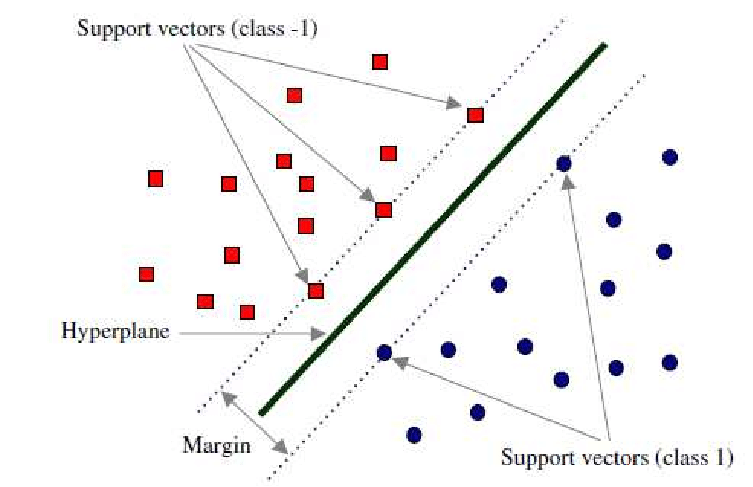
\includegraphics[width=\columnwidth]{../Figures/SVMpic}
\caption{SVM seeks to maximize the margin as shown on the figure. This is done by separating the two classes by a hyperplane. Note that although this is a 2D depiction of SVM, the algorithm can be applied to n-dimensional space. \label{figure:SVMex} \protect\citep{SVMPic}}
\end{figure}


Using these principal components, it is possible to apply SVM to this now dimension-reduced dataset to classify the data if it is linearly separable.  However, there are still some shortcomings with this method. Most importantly, SVM is only effective on linearly separable data---data which can be divided with a straight hyperplane like that seen in Fig.~\ref{figure:SVMex}---and real life data often is not. Therefore, more sophisticated methods such as the 'kernal-trick' \citep{kernaltrick} try to circumvent this problem by extending the algorithm to extra dimensions. However even with these methods to extend the applicability of SVM, it remains ineffective on some datasets. There are other classification algorithms such as logistic regression---see Sec.~\ref{sec:Logistic}, but they continue to be unable to classify all datasets generally \citep{UniversalApproximationTheorem}. Another downfall is with PCA. Due to the nature of dimension reduction, some data must necessarily be discarded. Even though the PCA algorithm guarantees that the minimum amount of data will be discarded by virtue of ordering all the principle components in descending variance, for a given principal component selection, some is discarded nonetheless. If one's computing power allows, it is clearly superior to not discard any data at all. 

The next step in the field of machine learning happened relatively recently---developing to the current form the last 5 years---and is mainly due to advances in hardware as well as breakthroughs in computer science. 

A neural network is a network which mimics the way a biological brain works---with an array of mathematical nodes (otherwise termed neurons to draw a parallel with the biological equivalent), which are connected to each other in some way. 

The use of a neural network has been discussed for some time before its prevalence in computer science today \citep{History}, in fact a SVM classifier can be seen as a prototype of neural networks (a type of basic neural network called a perceptron). However, for a long time, deeper---i.e. neural networks with more intervening layers between input and output---neural networks were hampered by a lack of ability to train them effectively due to convergence issues with optimisers, essentially rendering those types of neural networks untrainable.\citep{History} When this issue was solved, the field of machine learning was also aided by the exponential growth of processor speed, which allowed more complex (deep) neural networks to be designed and trained.

There were a subsequent two problems to be solved before machine learning---the use of algorithms which naturally improve---could be used: the unstable-gradient problem (also known as the the vanishing-gradient problem in certain instances) was solved using further backpropogation (see Sec.~\ref{sec:BP} because hardware advances allowed this; and a shift of activation function because sigmoid functions sometimes cause a saturation in the final hidden layer---the final layer before the output node---\citep{ReLu}, this was remedied by using another activation function (ReLU function, see Sec.~\ref{sec:ReLU}) that is now ubiquitous in modern neural networks. This allowed deep convolutional neural networks to be used efficiently and thereby resulting in the rapid development of the field of Computer Vision (recognising images using computers). \citep{NeuralNetworksandDeepLearning}

The primary goal of this project is to create a classifier that could classify sources on the image into stars or galaxies. The secondary goal was to extend that classifier to discriminate between spiral and elliptical galaxies. 

This project approached this problem from a largely computer science perspective and therefore the techniques used stem from current techniques in computer science. 

\section{Theory}

Given that the project is a synthesis of the fields of survey astronomy and machine learning, many of the terms and techniques used will be unfamiliar to astronomers who have not worked in the machine learning field. This section seeks to give an overview of the important parts which are necessary to understand this project. 
\subsection{Classifiers}
\label{sec:classifier}
A classifier is defined as an algorithm which predicts the class of a datapoint. A classifier can be seen as approximating a mapping function $f$ from input variables $X$ to discrete output variable $y$. N.B. In machine learning, these variables may be matrix or tensor objects. A datapoint here simply means an instance of $X$ which the classifier needs to classify.  Within this project, the datapoint is a single image cutout, and the output is a determination whether the image is of a star or a galaxy. 


\subsubsection{Logistic Regression/Sigmoid Activation Function}
\label{sec:Logistic}
Logistic regression was previously the preeminent binary classification algorithm in use due both to its simplicity, as well as its properties which are very conducive to gradient descent optimization as detailed below. The function used in logistic regression is the sigmoid function, which is used as an activation function in neural networks. The sigmoid function was used as an activation function in the CNN variant of neural networks used in this project. \citep{LogisticRegression}

The logistic regression algorithm attempts to split a dataset into two classes---a positive class represented by an output of 1, and a negative class represented by an output of 0. It uses the sigmoid function to do so.
\begin{equation}
h(X)=\sigma(Z) \textnormal{, where } \sigma(Z)=\frac{1}{1+e^{-Z}}
\end{equation}
h is a linear parameter which broadly speaking gives the probability that 'X' is in the positive class. 
From the above, it is clear that $\lim_{Z \to +\infty} \sigma(Z)=1$ and $\lim_{Z \to -\infty} \sigma(Z)=0$. This allows for the classification of X based on inputs to Z. 

As stated above, $X$ is a generalised variable representing all the features(variables) $\{x_1,x_2,x_3,...\}$ that are inputs to the sigmoid function. Therefore X is a (usually column) vector.

The formal definition of the sigmoid function in the context of logistic regression is 
\begin{equation}
	h_\theta(X)=\frac{1}{1+e^{-\theta^T X}}
\end{equation}
In Machine Learning the variable $\theta$ often denotes the weights applied to the generalised variable X to correctly predict the outcome. The $\theta^T$ in the exponent denotes the transpose of $\theta$ because $\theta$ is a column vector like X and so to multiply each weight by the appropriate variable, the transpose must be taken. N.B. An equivalent operation here is the dot product $\theta \cdot X$, however this is not usually used because it generalises poorly when multiple output $y$ are needed, i.e. when $y=\begin{bmatrix} y_{1} & y_{2} & y_{3} &\hdots \end{bmatrix}^T$. Note that $y$ is customarily notated as a column vector although the mathematics would be similar if it was a row vector.

The precise details on how to train a logistic regression model is beyond the scope of this report, but broadly speaking, a $\theta$ is found such that it correctly predicts the class of any given X. 

The sigmoid function is just a function that takes inputs from $-\infty$ to $+\infty$, and outputs a number between 0 and 1. In the case of logistic regression, this can be seen as a probability that the input belongs to either class. In more complex neural networks, this function can play the role of an activation function. An activation function is just a function which processes the inputs taken from one or multiple nodes and outputs it to some other node. The activation function itself resides within a node and has some node weight $\theta$ related to it. 

A sigmoid function was ubiquitous as an activation function before 2011 because it satisfies a few requirements that make such an activation function very useful. It is nonlinear, which enables a two layer network to be a universal approximator by way of the Universal Approximation Theorem \citep{UniversalApproximationTheorem}. A universal approximator is a mathematical idea of a network can approximate any mapping function which includes the classification function as described in \ref{sec:classifier}. In practice, like many theoretical ideas, this is never reached, and more layers are necessary. However, it is key to note that any number of  linear activation may \textit{not} be a universal approximator. The sigmoid function is also continuously differentiable which makes a gradient descent approach---a very common way of optimising a neural network---possible. However, it fails in some circumstances such as saturating the final hidden layer which renders it unusable \citep{ReLu}. Therefore the field of machine learning has steadily shifted away from using sigmoid activation functions.

\subsubsection{Rectifier/Rectified Linear Unit}
\label{sec:ReLU}
A rectifier is just like a sigmoid function in that it serves as an activation function in a node. The rectifier function is defined
\begin{equation}
f(x)=\textnormal{max}(0,x)= \begin{cases} 0, & \mbox{for } x\leq0 \\ x, & \mbox{for } x>0 \end{cases}	
\end{equation}
This function was found in \citep{ReLu} and it quickly became the favoured choice of activation function for neural networks. In the same paper, it was shown that this function also satisfies the non-linearity requirement. This function is not differentiable everywhere though, its derivative at 0 is undefined. However there are two solutions to this: the analytic solution is to define the derivative as 0 or 1, since those are the values of the derivative of the function elsewhere---0 for $x<0$, 1 for $x>0$. If this derivative at 0 is defined, then the derivative for the function is continuous. The second solution is that in a practical context, a node would never reach 0, because of the nature of gradient descent, the local minima is never actually reached, there is always some small value above or below 0, therefore the issue of an undefined derivative is not reached. Finally, this activation function has the added benefit of having an infinite range: $(0,\infty]$, which increase the speed of convergence of a model. NB: Convergence in machine learning refers to the behaviour of a neural network to reach a minimum of loss function. An algorithm which converges slowly requires longer (in terms of epochs) to reach this minimum than one which converges quickly. An algorithm which does not converge does not reach a minimum, not even a local minima.

\subsection{Neural Networks}
A neural network is a set of nodes (which include the aforementioned activation functions) arranged in a certain way. Pertinent to this project is the feedforward neural network (FNN) and the convolutional neural network (CNN) as those are the networks used.
\subsubsection{Feedforward Neural Networks}
Feedforward Neural Networks (FNN) are a type of network which was initially attempted in this project.

A feedforward neural network (FNN) is a neural network only feeds data forward through the network, i.e. there are no loops. This is the most simple type of neural network but it is also the most versatile. Because the inputs can be any type of numerical data, of any dimension, the neural network can approximate any function required (Universal Approximation Theorem) \citep{UniversalApproximationTheorem}. Formerly, an FNN may only have 1 hidden layer (HL) which is due to both problems with training a neural network with anything more than 1 HL (backpropagation \citep{Backpropagation}), but also due to nomenclature: anything with more than 1 HL is called a deep feedforward neural network. With the advent of much more powerful hardware and also techniques to effectively train multi-layered neural networks, these 'deep' feedforward neural networks replaced single-layered neural networks in almost all applications. Thence, all of these neural networks were generically termed 'Feedfoward Neural Networks'.  \citep{FNN}

\begin{figure}
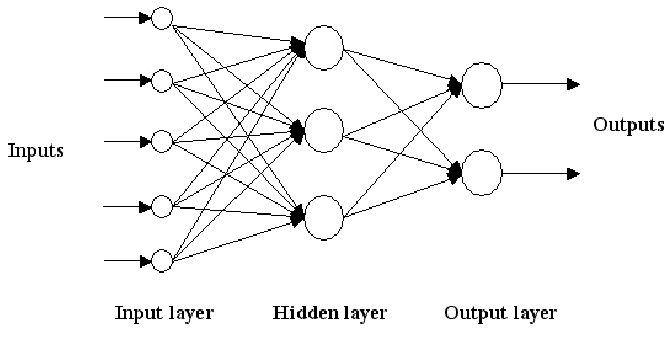
\includegraphics[width=\columnwidth]{../Figures/FNN_Diagram}
\caption{This is a schematic diagram of an FNN. Note that the input layers are more numerous than the outputs. Also note that the connections between nodes in the layers are all pointing towards the output direction---the eponymous 'Feedfoward' in feedforward neural network. The Hidden Layers (HL) are so termed because one external to the neural network does not directly interact with that layer. One would provide inputs as take outputs, but does not see the workings of the intervening layers, hence their name as 'hidden layers'. \protect\citep{FNN} \label{fig:FNN_Diagram} }
\end{figure}

An FNN has nodes in those layers and the number of nodes in those layers vary by network architecture. Broadly speaking those nodes act take outputs from previous nodes and put them through an activation function initially defined (nowadays usually ReLU, sigmoid less commonly seen). This activation function outputs a value which is in turn passed to the next node.

At the end of the FNN, there is an output layer of nodes which returns the output which the classifier is meant to produce. In this project, the output is a single node which outputs a number to indicate whether the FNN predicts the class of the ingested image to be a star or galaxy.


However, the performance of FNNs in classifying images was not satisfactory which was why the focus of the project turned to CNNs.

\subsubsection{Convolutional Neural Networks}
\begin{figure}
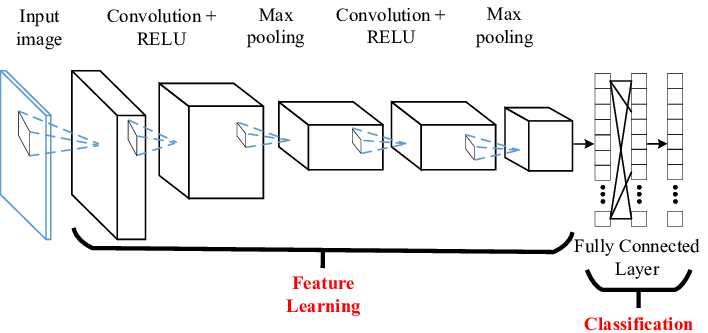
\includegraphics[width=\columnwidth]{../Figures/CNNdiag}
\caption{A schematic diagram of a CNN showing all the main features which include convolutional layers, pooling layers, and classification layer(s). Note that the dimensions of the image get decreased during the feature learning process. This is both a natural consequence of the convolution operation as well as a intended consequence of using pooling layers. \protect\citep{CNNdiag}\label{figure:CNNdiag}}
\end{figure}


A significant downside of FNNs is that in the course of ingesting data into the neural network, one must flatten the 2 dimensional data into a 1 dimensional vector.
For example, given image data of 2 dimensions in matrix form X, the matrix must be compressed in this way:
\begin{equation}
	X=\begin{bmatrix}
           x_{11} & x_{12} & x_{13}\\
           x_{21} & x_{22} & x_{23}\\
           x_{31} & x_{32} & x_{33}\\
         \end{bmatrix}
         \rightarrow \begin{bmatrix}
           x_{11} \\ x_{12} \\ x_{13} \\
           x_{21} \\ \vdots \\ x_{33} 
         \end{bmatrix}
\end{equation}
Any and all subsequent operations on each of the elements can then only take into account the value within the column vector. This prevents the nodes from taking into account the surrounding pixels of the pixel which the node is acting on. This loses vital information about edges, corners and other visual aspects of images on the scale of 'a few' pixels which are vitally important to be recognised. This motivated the development of the convolutional neural network (CNN).

A CNN, strictly speaking, can be thought of as a type of FNN due to it not having any recurring loops. However, in practice it is generally thought of as distinct due to it having vastly different node behaviour. 


A CNN, like its name suggests, is a neural network which has nodes which perform convolutional operations. A general CNN diagram can be found in Fig.~\ref{figure:CNNdiag}. Convolution is most often approached in physics in terms of a signal being convolved with a background. This is essentially the same operation that a convolutional node performs. A convolutional filter is applied to an image, this consists of a kernel which describes the function---which is almost always a linear shape---that passes over the original image and passing the result into a new image. This concept is easier explained visually, see Fig.~\ref{fig:convolution}.

\begin{figure}
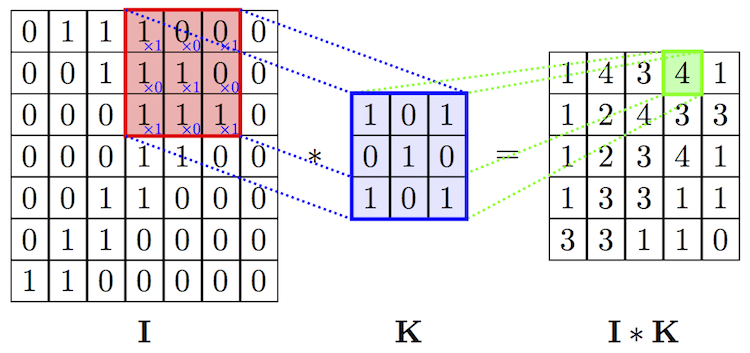
\includegraphics[width=\columnwidth]{../Figures/convolution}
\caption{The convolution operation involves an incoming array(matrix) which is labeled \textbf{I} in the diagram. The convolution kernel (labeled \textbf{K}) is moved over the incoming array and each of the corresponding values is multiplied and output to an ouput array \textbf{I$\ast$K}. Since the value in the output array is placed in what would be the center value of the kernal, the dimensions of \textbf{I$\ast$K}is smaller than \textbf{I}. \protect\citep{convolution}\label{fig:convolution}}
\end{figure}

A CNN has 3 types of layers: convolution layers, pooling layers, and a fully connected layer. A convolution layer performs a convolutional operation as described above. It has 4 key parameters: kernel, stride length, layer size, and activation function. The kernel describes the kernel which is passed over the incoming image, the key parameter of the kernel is the size---kernels are usually squares of 3x3, 5x5, or 7x7 size, with the size determining how many neighbouring pixels one wants the filter to take into account. The stride length is how many pixels the filter jumps over before the next filter is applied---i.e. if the stride length is 1, then every pixel will have the filter applied, while if the stride length is 2, then every other pixel will have the filter applied. The layer size is how many convolutional filters are passed over the incoming image. Because each nodes has different initial conditions, this represents the trainable part of the network. Finally, the activation function determines what value is outputted to the subsequent layer. In a modern CNN it is usually ReLU due to it working better with sparse models. \citep{CNNSparse}

A pooling layer can be thought of as a specific type of convolutional layer in that the kernel is a flat one. Its main purpose is to reduce the dimension of the incoming image. 

\begin{figure}
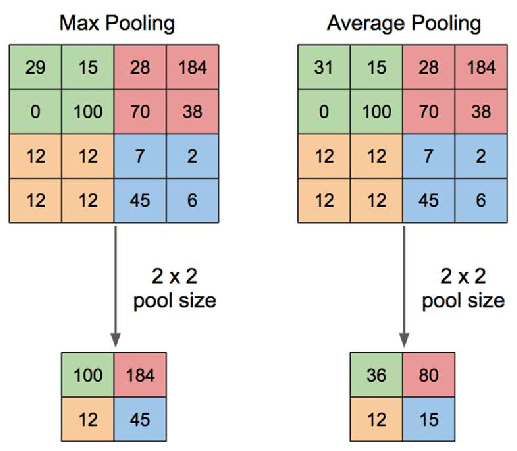
\includegraphics[width=\columnwidth]{../Figures/pooling}
\caption{The pooling operation involves reducing the size of the incoming image by either taking the average of a group of pixels or the maximum value of a group of pixels. Both methods are depicted above. The max pooling method is generally seen as superior. \protect\citep{pooling}\label{fig:pooling}}
\end{figure}


There are two types of pooling layers: average pooling and max pooling. An average pooling layer inputs the average value of the pixels within the pooling filter and outputs them to the next image. A max pooling layer does essentially the same but with the maximum value of the pixels rather than the average value. This achieves the same amount of dimensionality reduction except the max pooling layer achieves noise suppression by discarding the noisy activations. The max pooling layer is therefore said to be superior to the average pooling layer. See Fig.~\ref{fig:pooling}. 

Fully connected layer(s) are simply an FNN added in the end of the convolutional layers used to gather the results of the convolutional and pooling layers and output to a visible layer, of which the results can be used. The complexity and size of the fully-connected layers vary depending on the task---in the current project, a single node at the end of the convolutional and pooling section of the network is sufficient. In binary classification cases a binary activation function such as sigmoid, ReLU, or tanh can be used, while in multiple-class classification problem a function like softmax---a generalization of the sigmoid function to multi-class---should be used instead. \citep{Goodfellow-et-al-2016} 


\subsection{Optimisation algorithms}
In order for a neural network to be of any use to anyone it must be trained. Training is a process where the weights of the neural network are modified to better predict the desired outcome. The broad idea behind optimisation of a neural network is that one is trying to minimise some loss function. A loss function is a function assigned to assess the classifier. There are many varieties of loss functions, but a simple example of one would be a function that assigns a loss of 1 when a classification is incorrect while a loss of 0 when the classification is correct. The optimizer will then seek to change the classifier in such a way to minimize this function. 

Given that the problem is a minimisation problem, it would be reasonable to use some kind of algorithm which takes into account the gradient of the hypersurface that the optimiser is attempting to optimise over because it is known that at local minima the gradient of the surface is 0. In fact, descending via gradient descent ensures that the path descended is the steepest one. \citep{Gradient Descent} NB: A hypersurface is a generalization of the concept of the surface which exists in 3D space. A surface is a 2D object which exists within a 3D space, similarly, a hypersurface is a (n-1)D object in n-D space. 

In a general form, the equation for gradient descent is 
\begin{equation}
\theta_{n+1}=\theta_{n}-\alpha\nabla J(\theta)	
\end{equation}
where $\theta$ is a general set of weights applied at any particular node. $\theta_{n}$ is the set of weights before updating while $\theta_{n+1}$ is that after updating. $\alpha$ is a variable called the learning rate, which controls how 'far' in any one direction one update moves the weights on the hypersurface. $\nabla J$ is the key term here as this is the gradient of the cost(loss) function over all variables which ensures all the weights for the variables are updated in the same pass. \citep{GradientDescent}

\subsubsection{Backpropagation}
\label{sec:BP}
An aside must be made to briefly discuss backpropagation which was instrumental in allowing deeper neural networks to be trained. 

The above gradient descent technique applies to one single node. Modern neural networks have multiple layers each containing many nodes. What the gradient of each node is unclear for the hidden layers due to no one being specifically responsible for the output. 

Backpropagation solves this problem by relating the error (and hence gradient) of each of the node to the partial derivatives of the error of the nodes in the preceding layer. This propagates the errors backward though the neural network enabling the network's weights be trained via gradient descent. The exact mathematics of backpropagation is far beyond the scope of this report, for more robust mathematical discussion see \citep{Backpropagation}.

\subsubsection{Stochastic Gradient Descent}
Because of the large datasets often used in machine learning, it is impractical to use the whole dataset at once as is required in gradient descent, not least because of memory constraints inter alia. Therefore, a new algorithm---stochastic gradient descent---was developed to train using these large datasets.

Stochastic Gradient Descent (SGD) is an algorithm which chooses a random input datapoint within the whole dataset to perform the gradient descent algorithm. This was developed due to the need to train larger and larger datasets. Larger datasets present a challenge due to the longer time it takes to calculate losses through the entire dataset, at some point large datasets present a hardware constraint of not having enough RAM to store the entire dataset in memory which makes gradient descent through the whole dataset unworkable. 

SGD solves this by updating the weights after a single datapoint. This allows the weights to converge much quicker than in normal gradient descent. However, because each datapoint updates the gradient this introduces a lot of noise which cannot be removed. A modern compromise is to use mini-batches---updating the weights after every few 10s or 100s of datapoints. \citep{SGD}

\subsubsection{Momentum}
A modern advancement to the gradient descent algorithm which is almost ubiquitous in all modern optimisers uses a concept called momentum. The full mathematical treatment of momentum is beyond the scope of this report, but a general explanation of the concept will be given. \citep{Momentum} The general concept of momentum is the addition of a variable $v$, representing the momentum of the descending 'particle'. The updating equations are changed to 
\begin{equation}
\begin{cases} v_{n+1}=\eta v_{n}-\alpha\nabla J(\theta)  \\ \theta_{n+1}=\theta_{n}+v_{n+1}\end{cases}
\end{equation}
with $v$ being the new momentum parameter and $\eta$ being a new decaying hyper-parameter. This has the effect of both accelerating convergence due to the momentum term accumulating a large value from repeated updates in the same direction; and the effect of smoothing out noise because local fluctuations in gradient get smoothed over by the overriding momentum term.

\subsubsection{Modern Optimisers}
\label{section:modern optimizers}
Modern optimisers tend to use an adaptive learning rate. The learning rate $\alpha$ as described above in the aforementioned optimisers are constants. However it is often advantageous for the learning rate to change with respect to the parameters.
 
 The first modern optimiser in this regard is Adagrad (for 'adaptive gradient') published in 2011. \citep{AdaGrad} This implementation adds the adaptive gradient using a multiplicative term in the denominator that sums the squares of previous gradients. This method allows the learning rate to be greater in the beginning of training where, presumably, the parameters are further from the minimum; and decreasing as the minimum is approached. Adagrad reduces the learning rate according to the size of all previously-calculated gradients (i.e., so large gradients lead to slower rates). A downside of Adagrad is that the learning rate decreases so much near the minimum that minimum itself is never reached, especially if early gradients are very large. The Adadelta optimiser attempts to solve this by only considering more recently-calculated gradients, and so excludes the large gradients encountered at the start of learning. \citep{AdaDelta}

 Adam (for 'Adaptive Moment Estimation') is an algorithm which is a development from Adadelta and another algorithm called RMSprop, which remains unpublished as of the time of writing. Like Adagrad, the Adam optimiser considers all previous gradients when calculating the learning rate. However, it downweights via an exponential function (rather than ignoring entirely) earlier gradiants so to avoid reducing the learning rates to overly low levels. In addition to the square of the past gradients that AdaDelta and AdaGrad stores, Adam also stores an average of past gradients which is used to implement the momentum aspect of the algorithm. Because of the momentum implementation, Adam generally displays faster convergence compared to AdaDelta. These are then used to update parameters similar to the above methods. \citep{Adam} Adam has become the dominant optimiser for neural networks within computer vision and natural language processing due to the result being favourable in comparison to other optimisers. As such, Adam is the chosen algorithm for optimisation within this project.
 

 \begin{figure}
 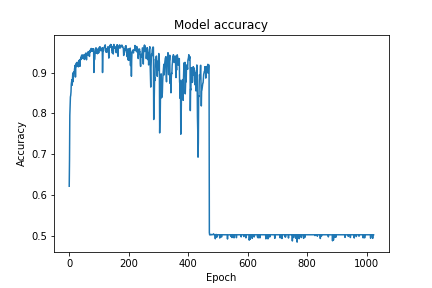
\includegraphics[width=\columnwidth]{../Figures/CNN_zeroing_accuracy}	
 \caption{An example taken from a training run of a neural network using the Adam Optimiser without the AMSGrad adjustment. The accuracy of the classifier first rises to over 0.9, then drops precipitously to an accuracy of 0.5. An accuracy of 0.5 represents a classifier which is no better at classifying than random chance. This is thought to be caused by the momentum causing an overshoot of the minimum. \label{figure:zeroing}}
 \end{figure}

 However, adaptive learning rate optimisers have the downside of not converging in certain circumstances. See Fig.~\ref{figure:zeroing}. The detailed reason can be found at \citet{ObjectAMSGrad} and \citet{translateAMSGrad}. In 2018, \citet{AMSGrad} has modified the Adam algorithm where instead of always using an exponentially decaying average, it uses either the current squared gradient (calculated using the exponentially decaying average as before) or the past squared gradient immediately preceding, whichever is greater, to determine the learning rate and the momentum. This results in the step size of AMSGrad never increasing, which avoids the problem found in Adam. This algorithm is called AMSGrad and the authors have included a proof of convergence that Adam lacks. This algorithm outperforms Adam on small datasets while shows similar or worse performance on other datasets. Since this algorithm is very new, it is yet to be determined if this algorithm is superior to Adam.
 
 
 \begin{figure*}

 \begin{subfigure}{0.666\columnwidth}
 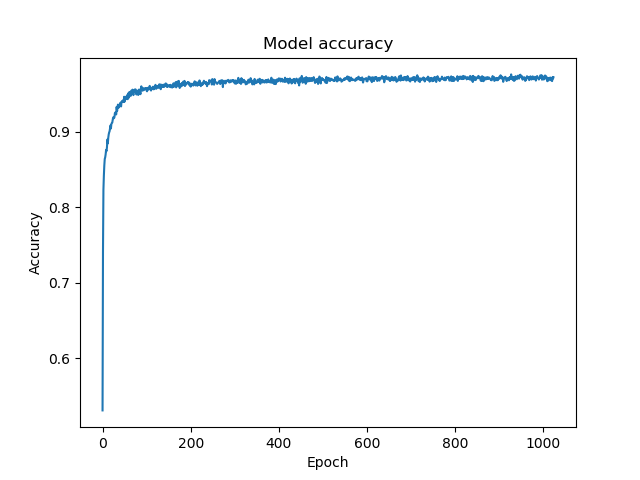
\includegraphics[width=\columnwidth]{../Figures/FNN_AdaDelta} 
 \caption{AdaDelta}
 \label{fig:AdaDelta}
 \end{subfigure}
 \begin{subfigure}{0.666\columnwidth}
 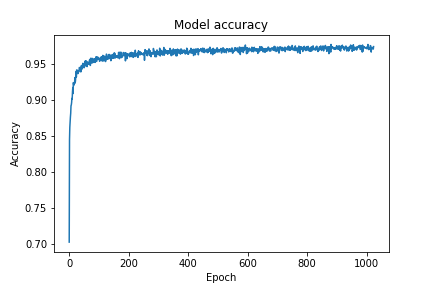
\includegraphics[width=\columnwidth]{../Figures/FNN_Adam}
 \caption{Adam}
 \label{fig:Adam}
 \end{subfigure}
 \begin{subfigure}{0.666\columnwidth}
 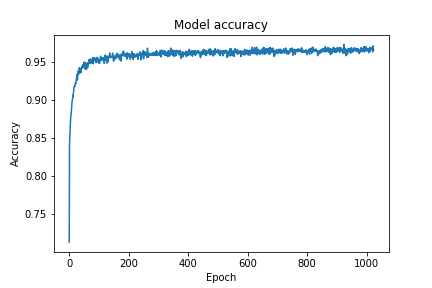
\includegraphics[width=\columnwidth]{../Figures/FNN_Adam_AMSGrad}
 \caption{Adam with AMSGrad}
 \label{fig:AdamAMSGrad}
 \end{subfigure}

 \caption{The three optimizers tried in this project is AdaDelta, Adam and Adam with AMSGrad. Adam represents a significant improvement over AdaDelta in convergence speed, however sometimes fails to converge at all in some CNN cases (See Fig.~\ref{figure:zeroing}). The AMSGrad algorithm appears solve that problem at the expense of some extra variation during convergence. Therefore Adam with AMSGrad is chosen as the optimizer for all the neural networks in the project.}
 \label{fig:Optimizers}
 \end{figure*}

\section{GOTO}
The proximate cause for this project and hence report is that the Gravitational wave Optical Transient Observatory (GOTO) records a very large amount of data which needs to be classified. Because the amount of data is too large for any human to complete in any reasonable amount of time, machine learning was enlisted to solve this problem. \citep{GOTO}

GOTO is an observatory which is primarily used to record the optical emissions from phenomena associated with gravitational wave events. However, when no gravitational wave events require active follow-up from GOTO, it has a secondary mission of performing survey astronomy. 

Each GOTO observation is undertaken with a complement of up to 8 Unit Telescopes (UT) which are slightly offset from each other to observe more of the sky at once. Each of these UTs have a field of view of around 6 sq. degrees. 

\subsection{Data Pre-Processing}
The data used in this project was preprocessed using the LSST stack. The steps involved in the preprocessing are:
\begin{itemize}
\item Constructing master calibration frames from bias, dark, flat frames on observations made over several nights
\item Removing the noise in science frames using these calibration frames
\item Cosmic ray removal
\item Background subtraction
\item Modelling the point squared function of the science frame
\item Calibration of the image by comparison to external catalogues
\item Source detection, deblending, and measurement on each science frame
\item Frame alignment and coaddition
\item Forced photometry using the coadded frames
\item Comparison to the previous images to determine if the sources have changed
\end{itemize}

The exact way the data is processed is detailed in \citet{LSST} 
and \citet{GOTOLSST}. 


 \section{Method}
The method of making a working classifier relies has 3 parts. First, cutouts around each object within the larger GOTO images must be made. These need to be split into galaxies or stars for labelling. Second, a neural network architecture must be decided on and the cutout images are used to train this network. Finally, the classifier evaluated using the test dataset.
\subsection{Cutout Algorithm}
The initial .fits files from GOTO are 6132$\times$8176 pixels in size, and to prepare the images for training in a neural network, some preprocessing of the data is needed. 

A cutout algorithm was written for this. Since the images provided have already been processed, the science layer within the .fits file is assumed to be the true pixel intensity values and will be worked with directly. The values are directly extracted with to a data array (\texttt{ndarray} from \texttt{numpy} package).

\subsubsection{Source Detection}
The first step in the data processing is to perform source detection on the data. Source detection is performed using the  \texttt{detect\_sources} function within the \texttt{photutils} package. This function requires data, threshold, number of pixels and the filter kernel. The filter kernel is a smoothing algorithm that smoothes the incoming data by passing it through a kernel. In this case, the kernel is defined to be to cause the signal to be smoothed to a full-width half-maximum of 3 pixels. This helps the detection algorithm detect sources because the algorithm relies on contiguous pixels to detect sources and smearing out some light onto nearby pixels assists allows very small sources as well as artefacts to be detected.

The next input is the threshold which defines the limit at which the sources will be detected. This threshold can be an absolute value for which the source must have a certain intensity to be detected. However, this fails to take into account the background of which the source lies on. Therefore, in the current implementation the background is taken into account by creating an estimated background using the \texttt{Background2D} function, also within the \texttt{photutils} package. This estimates a background of the image given some parameters and the data of the image. The key parameters is the box size, which determines across how many nearby pixels should the background be considered to be constructed over---in this case it is a 50x50 box which is reasonable given that the surrounding 25 pixels in each direction should give a good estimate of the local background of the source. Normally this box should be a divisor of both the total x and y pixels in the entire number due to edge effects that would be an issue if fractions of boxes are left at edges. Here, this is not an issue because the cutout algorithm---as shall be explained below---cuts out the edges of the image, so this is a non-factor. This background estimator uses a median estimator which estimates the background based on the median value rather than an average value. \citep{photutils} This is so because where a source would exist, these represent much higher values than the background values and an average would wrongly 'drag' up the results due to sources which patently are not part of the background. Finally the threshold which enters the source detection algorithm is defined as 10 times the estimated background at the point. This means that for a collection of pixels to be defined as a source, the source detection algorithm requires that the number of contiguous pixels which all have brightnesses greater than 10 times the estimated background be greater than the number of pixels defined in \texttt{npixel}. This is a tradeoff between computing time and number of sources detected. If this number was lower, the number of detected sources would increase exponentially, but much more noise would also be detected hence causing a drastic increase in script runtime. Further, because of further steps such as cross referencing all the sources, this increase leads to further slowdowns in efficiency which is undesirable. However, having a much higher number would discard dimmer and more diffuse sources. This is particularly problematic because galaxies, in particular spiral galaxies, are particular diffuse and dimmer galaxies would be discarded which would lead to a lack of any galaxies to classify. Therefore, 10 times the estimated background is the tradeoff made here. See Fig.~\ref{figure:twotailed}

\begin{figure}
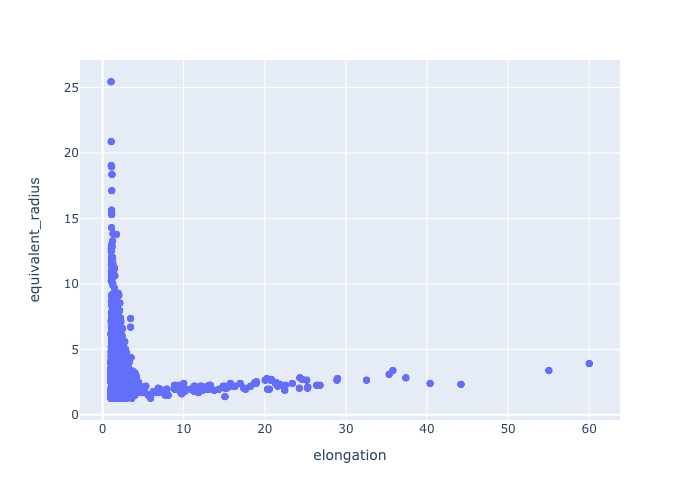
\includegraphics[width=\columnwidth]{../Figures/twotailed}
\caption{From plotting the two features of equivalent radius and elongation, there are two 'tails', corresponding to high equivalent radius and low elongation, and high elongation and low equivalent radius. The objects with high equivalent radius but low elongations are thought to be stars, while their counterpart are thought to be artefacts. Therefore it was decided that any objects with elongation over 10 should be discarded. \label{figure:twotailed}}	
\end{figure}

The number of contiguous pixels \texttt{npixels}, as mentioned above, is the number of contiguous pixels which all exceed the threshold. In the function \texttt{detect\_sources}, the default behaviour of this detection is that it considers all pixels which are side- or corner- connected to a pixel is considered contiguous---this is called 8-connected pixels and is left as-is in this implementation. 

The data which is inputted to the \texttt{npixels} is simply the raw data from the data array.

There is an additional step possible in this process which is to deblend the sources after detecting sources. Deblending is the process in which overlapping sources are distinguished from each other and listed separately. However, the current implement forsakes deblending for two reasons. First is that deblending is costly in terms of processing time---from experience adding the deblending step increases the processing time of the source detection part of the cutout algorithm by a factor of 5-10. While not an issue for the small scale of the current implementation, since the aspiration is for this to be applied to more data in larger applications of this algorithm, this processing time becomes significant and any savings in processing time is worth it. Second, because deblending deals with overlapping sources, this necessitates that the sources in question are actually overlapping. Therefore, any image-cutouts made from these sources are necessarily of both sources. Because of the implementation of this cutout algorithm also assigns classes (stars or galaxies), if two sources were overlapping and had one of each source, the result would be an entry of essentially the same overlapping source in each category which would present a problem in training the neural network eventually. 

The result of this is an object called a segmentation image. This object is an array with the same size as the data, but it marks pixels where a source is detected with a positive integer to indicate a source is detected.  This object is used in the \texttt{source\_properties} function and is called \texttt{segm} in the code. 

\subsubsection{Extracting Source Properties}
The data is then entered into the \texttt{source\_properties} function. This function takes primarily the data and the segmentation array as functions---it also takes World Coordinate System (wcs) information from the header which is required to reference the object's location in sky coordinates. This function outputs an object containing over 30 attributes containing the sources' properties. However, not all 30 attributes are relevant to this project---only 7 attributes are called: \texttt{xcentroid}, \texttt{ycentroid}, \texttt{sky\_centroid.ra}, \texttt{sky\_centroid.dec}, \texttt{elongation}, \lstinline{equivalent_radius}, \texttt{area}. 

Because the \texttt{source\_properties} function calculates the centroid and morphological features of sources \cite{sourceproperties}, the defining characteristics of the sources detected are the x and y positions of each source's centroid in pixel-space which are represented by the \texttt{xcentroid} and \texttt{ycentroid} values. Because the wcs of the original image is inputted to this function, it does a conversion to the the sky coordinates (right ascension and declination) of the sources, which are the \texttt{sky\_centroid.ra}, \texttt{sky\_centroid.dec} values. 

The elongation value is defined as the ratio of lengths of the semi-major and semi-minor axes. Elongation is defined thus,
\begin{equation}
\textrm{elongation} = 	\frac{a}{b}
\end{equation}
where a is the semi-major axis and b is the semi-minor axis.


 This metric is useful for determining the whether the the object in question is a true sky object or an artefact. 

The area is a measure of the area of sky covered by the source, it has units of pixel-squared. Determining the area is useful because it allows some determination to be made regarding tendencies for either stars or galaxies to be larger on the sky. It is not used in the cutout algorithm, but is retained for further investigation. The equivalent radius is a derived quantity from area, it is the radius of a circle with the same area as the source, it has units of pixels. 





\subsubsection{Data Cleaning}
Before the sources can be cut out individually, it is important that as many non-objects i.e. artefacts, be excluded from the extraction. This is done by excluding any source with elongation above 10. This number is a rough estimate to exclude any source which is clearly an artefact (See Fig.~\ref{fig:Examplefit}. All objects above elongation of 10 are clearly outliers while those under may or may not be.), but not too low as to exclude highly elongated sources, especially galaxies. 

Another aspect of the data that needs to be cleaned is that by observation of the image, there is a smearing at the edges of the image which elongates sources. This yields subpar samples to train with and therefore it is beneficial to exclude these sources. Therefore all sources which have centroids within 400 pixels of the left and right edges and within 300 pixels of the top and bottom of the image are excluded. 300 or 400 pixels are arbitrary numbers but they are approximately 5\% of the total sizes in either dimension. This means that approximately 10\% of the sources in either dimension are excluded this way. 

\begin{figure*}
 \begin{subfigure}{1.6\columnwidth}
 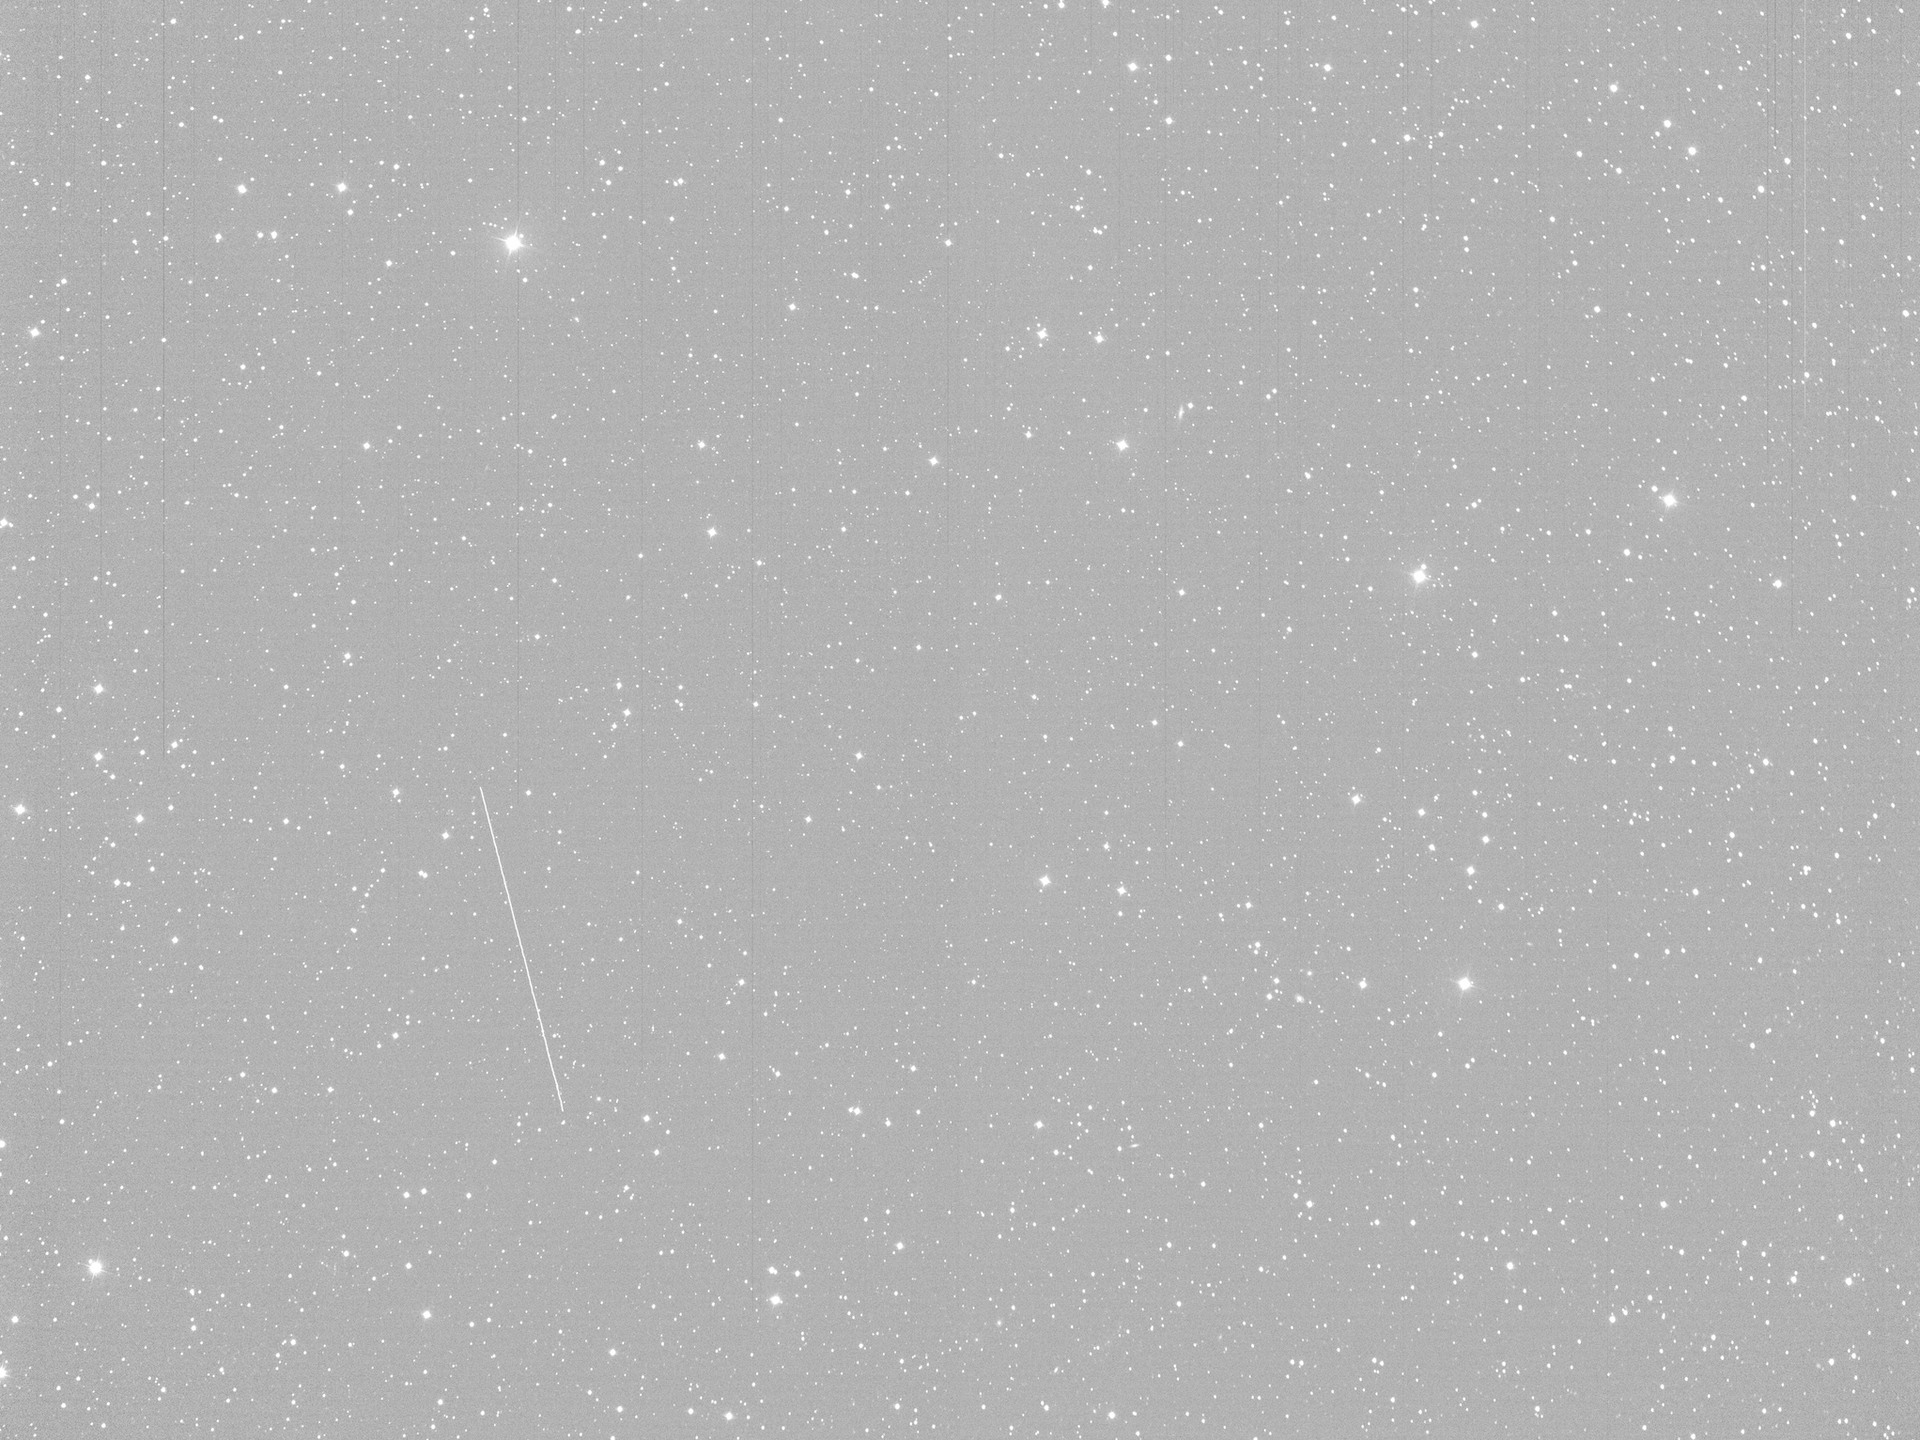
\includegraphics[width=\columnwidth]{../Figures/pic1} 
 \caption{asinh Scale}
 \label{fig:pic1}
 \end{subfigure}
 \begin{subfigure}{1.6\columnwidth}
 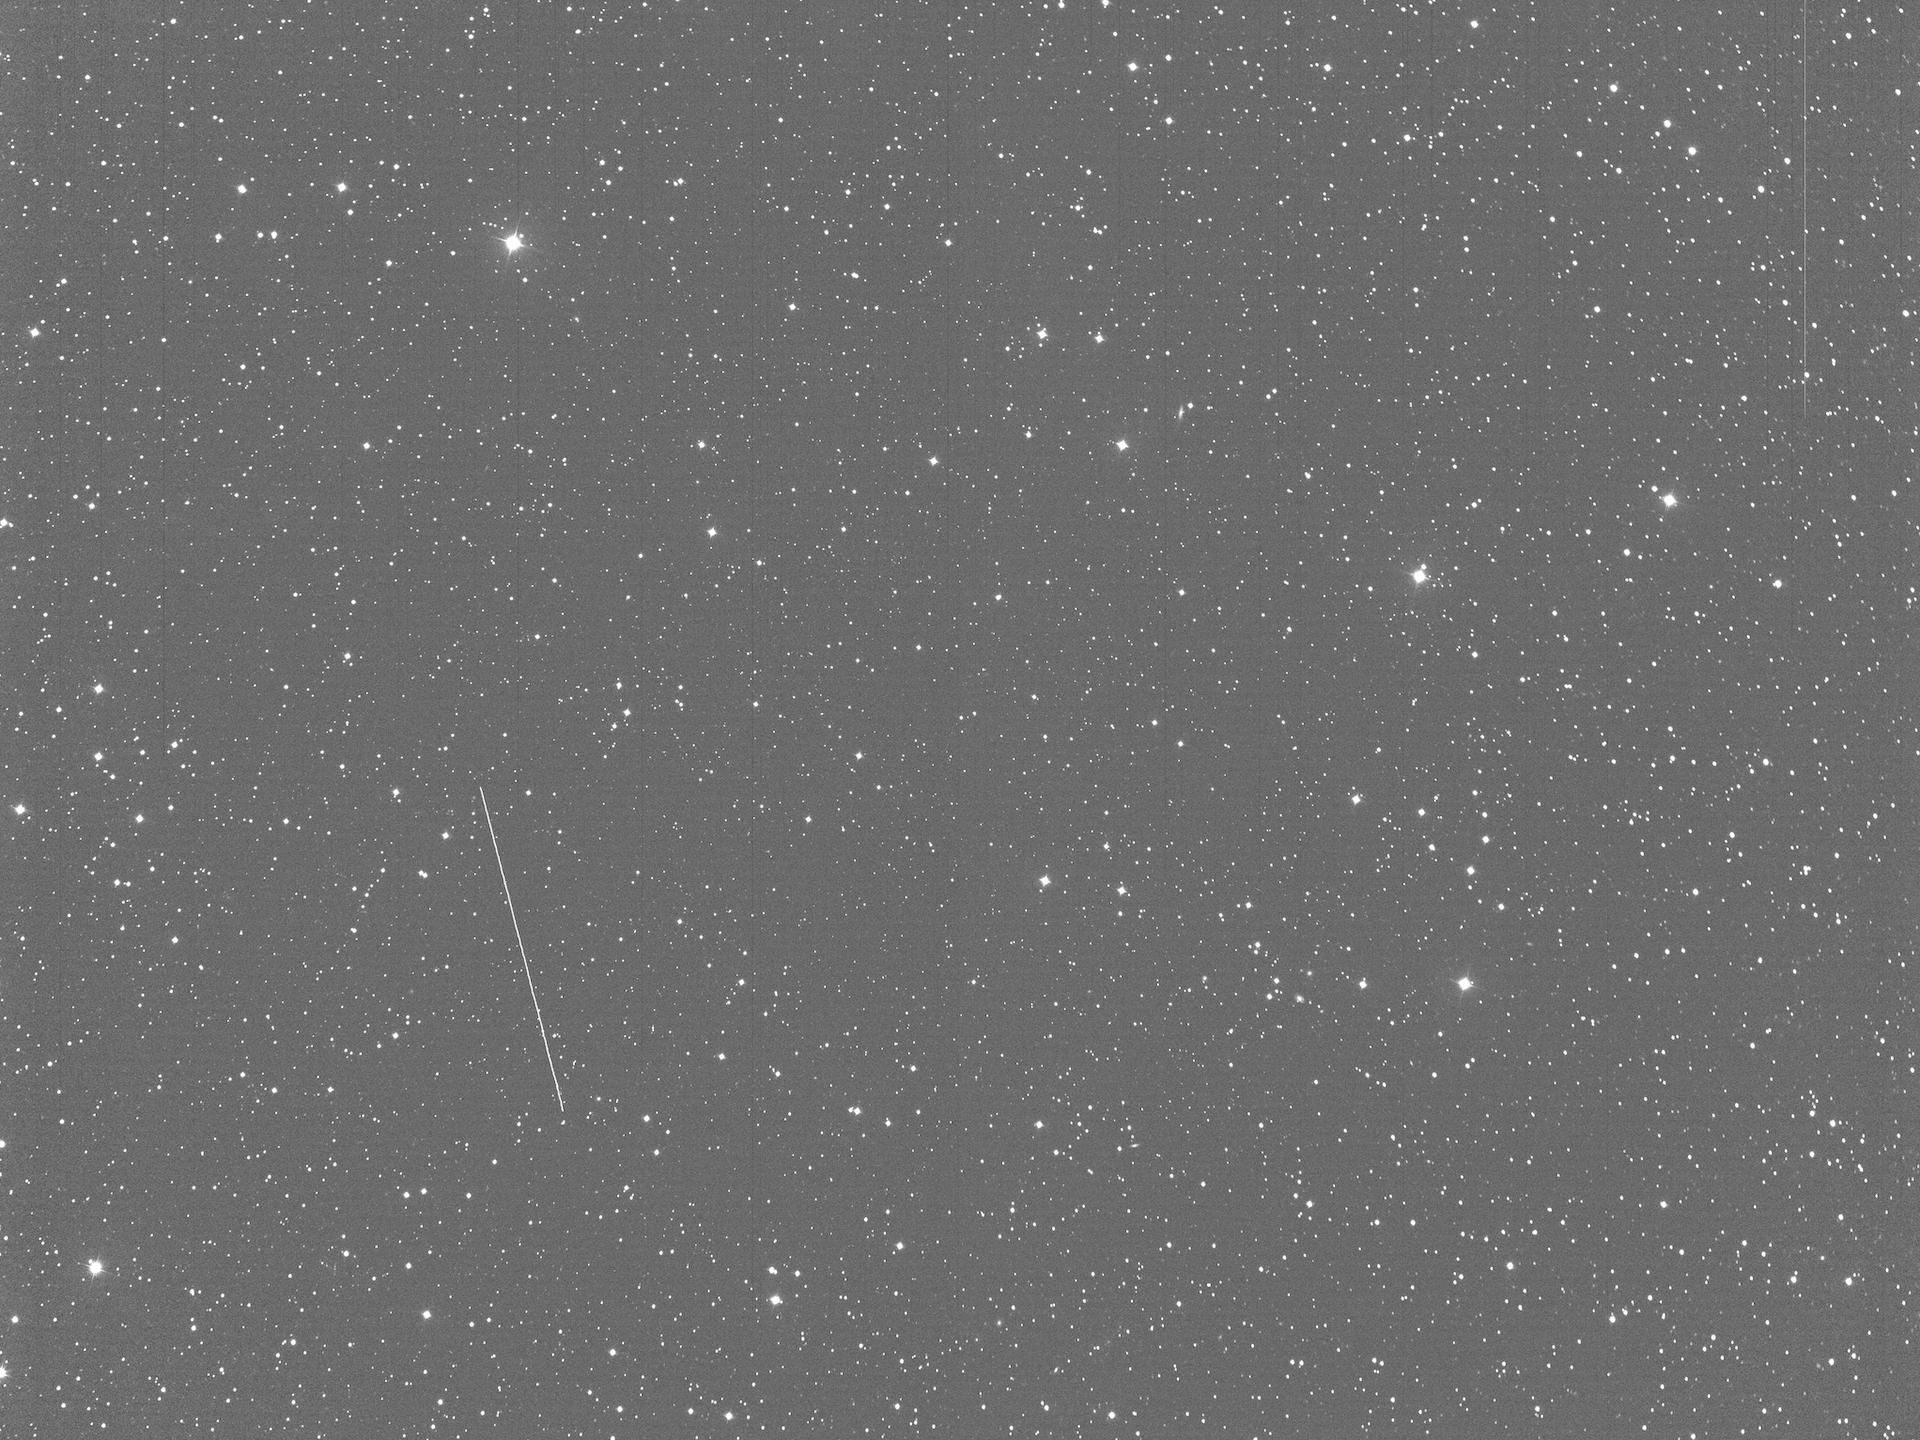
\includegraphics[width=\columnwidth]{../Figures/pic4}
 \caption{Linear Scale}
 \label{fig:pic2}
 \end{subfigure}

\caption{This is an example of an original image taken from a \texttt{.fits} file taken from GOTO after the initial processing. These are two different scales of the same image. Note that the edges of the images show some smearing of the objects---best seen in Fig.~\ref{fig:pic2}. There are also some dark vertical streaks in the left upper quadrant of Fig.~\ref{fig:pic1} which are artefacts of the telescope. These must be removed in the data cleaning stage of processing the image. There is also a bright streak which seems to be a meteor. Also note that the brightest objects in the image are stars and galaxies are hardly seen at all. \label{fig:Examplefit}}
\end{figure*}

\subsubsection{Database Matching}
Since labeled data is required for the training of the neural network, these labels must be acquired from a source external to the algorithm. In this project, labels are acquired from the SDSS database. 

To do this, a query within the \texttt{astroquery} package is made to the SDSS database. First, the algorithm requests all galaxies in the SDSS database with the constraints that: they are within the confines of the sky coordinates of the initial data image which is easily determined from the wcs data in the header of the .fits file, and that the galaxies are brighter than g-band magnitude 21. The magnitude threshold is an empirical determination based on number of sources returned---because the total number of detected sources from the image is determined beforehand, a magnitude which yields a similar number of sources should be correct. In practice, a selection that includes sources brighter than a g-band magnitude of 20 (i.e., $m_{\rm g}\leq20)$) results in too few sources, whereas $m_{\rm g}\leq22$ results in too many. Therefore $m_{\rm g}\leq21$ was deemed an appropriate magnitude threshold. 
This returns a list of sky coordinates which have galaxies matching the requirements. These sky coordinates are then matched against the sources detected using \texttt{astropy}'s matching algorithm and all matches with a tolerance of 3 arcseconds are cut out. 

The cutout algorithm is astropy's \texttt{Cutout2D}. The algorithm makes cutouts of the images, each with a size of 40x40 pixels. Each cutout is stored in a \texttt{.fits} file which is stored in a folder which contains to galaxies. The algorithm then appends modified header data into each cutout which makes it easy to find the location of a cutout from the original image if the need arises. 

The same procedure is completed for stars instead of galaxies with the results being stored in a dedicated stars folder. 

This part of the algorithm appears to be highly multithreaded. Using an 8-core Intel core-i9 9900HK running at 3.6GHz, it takes approximately 45 seconds for the algorithm to cut out each original image while it takes a 4-core Intel core-i7 6920HQ running 2.9GHz around 95 seconds on average. While there are some overhead losses, the performance seems to almost double with a doubling of the cores.

 \begin{figure}

 \begin{subfigure}{0.5\columnwidth}
 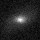
\includegraphics[width=\columnwidth]{../Figures/GalaxyExample} 
 \caption{Clear Galaxy}
 \label{fig:Galaxy1}
 \end{subfigure}
 \begin{subfigure}{0.5\columnwidth}
 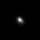
\includegraphics[width=\columnwidth]{../Figures/StarExample}
 \caption{Clear Star}
 \label{fig:Star1}
 \end{subfigure}
 \begin{subfigure}{0.5\columnwidth}
 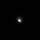
\includegraphics[width=\columnwidth]{../Figures/GalaxyExample2}
 \caption{Unclear Galaxy}
 \label{fig:Galaxy2}
 \end{subfigure}
  \begin{subfigure}{0.5\columnwidth}
 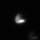
\includegraphics[width=\columnwidth]{../Figures/StarExample2}
 \caption{Unclear Star}
 \label{fig:Star2}
 \end{subfigure}

 \caption{A selection of the cutouts made from the cutout algorithm. Some objects, such as Fig.~\ref{fig:Galaxy1} and a lesser extent Fig.~\ref{fig:Star1} are clearly objects of their own classes. In particular Fig.~\ref{fig:Galaxy1} is clearly a galaxy (probably a spiral one at that) due to its central brightness and disky diffuse characteristic. However, Fig.~\ref{fig:Galaxy2} and Fig.~\ref{fig:Star2} are less clear in this regard. Fig.~\ref{fig:Galaxy2} seems that it could be just as well a point source and therefore a star and Fig.~\ref{fig:Star2} seems to be extended in appearance giving the impression of merging galaxies. However, they are a galaxy and a star respectively. This highlights the difficulty of classifying astronomical objects from morphology.}
 \label{fig:Examples}
 \end{figure}
 
\subsection{FNN}
The first step in making a neural network of any kind is to determine the network architecture. The network architecture is a description of the 'shape' of the neural network. The network architecture describes how many layers, and what type of layers exist between the input and output. It also describes the size of each layer---i.e. how many neuron/nodes a layer has. 

The FNN was built on the \texttt{Keras} package using the \texttt{Tensorflow} backend. \texttt{Keras} was chosen because it is a high level abstraction on building a neural network to such an extent that building a neural network is quite simple and hence more time can be devoted to optimizing the network and other matters. However, the approach described here is general enough that any other neural network package or in fact programming language can be used. 

The building a network architecture is not an exact science and is usually highly empirical and depends on the dataset. Over the few years that FNNs have existed, there are a few guidelines which are found to work well. First, a FNN should have the minimum number of layers and nodes possible to solve a given problem to the desired degree. The reason for this is twofold---one should minimise the number of layers to train because each layer represents additional computational time which is required to train a neural network. Another reason is that larger neural networks are very prone to overfitting and hence lack generality to be applied to other datasets. The empirical rule here is that the number of trainable parameters in any given neural network should be smaller than the number of datapoints in the dataset the network is trained over. 

Second, FNNs layers should be built in decreasing size. The size of a layer can be thought of as the dimension the data has at that point. And so the reason this rule exists can be generally be explained as FNNs compressing highly dimensional data into a 1D output should be done sequentially because there is not much purpose in re-expanding data into a larger dimensional space because the data could already be expressed in a lower dimensional space. This means that nothing is gained from having a non-strictly decreasing size. 

Third, non-linearly separable data should be treated with at least 2 hidden layer FNNs with non-linear activation functions. The reason for having at least 2 hidden layers is due to the Universal Approximation Theorem \cite{UniversalApproximationTheorem}, however, because the UAT describes a mathematical optimal situation, often more than 2 layers are used, but this gives the lower bound on the number of layers necessary. The requirement for non-linear activation functions is because it can be shown that an infinite number of linear activation unit layers are required to provide the result of a single layered non-linear activation unit and that it is impossible to do better---i.e. mimic multi-layered non-linear activation functions.

The FNN used in this project largely has these rules in mind when built. The FNN architecture is shown in Fig.~\ref{fig:FNNModel}. As seen, the architecture has size 256, 64, 8 feedforward layers in sequence with all activation functions being ReLU. This gives $256\times 64+64\times 8 +8\times 1 = 16904$ trainable parameters. This is higher than the total number of images used for training (4996 images).  However, this size of network is necessary because of the high input size (1600). This network has 3 hidden layers which is generally thought to be a good number of hidden layers for a general FNN classifier. 

\begin{figure}
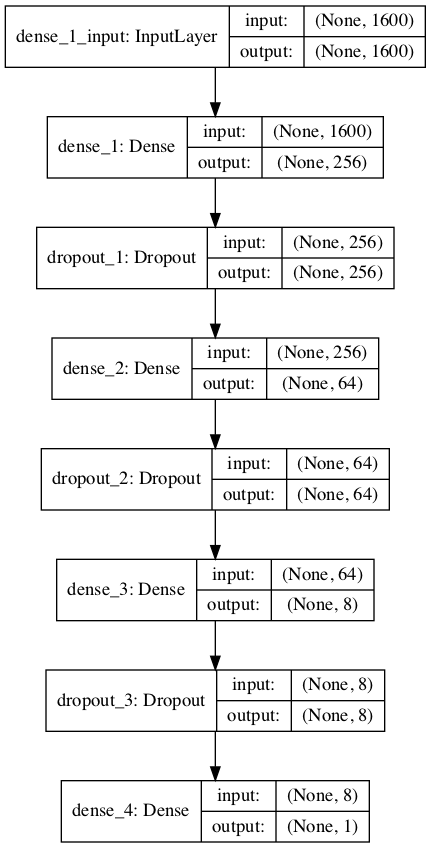
\includegraphics[width=\columnwidth]{../Figures/FNN_model_self}
\caption{The schematic diagram of the FNN architecture shows that there are 1600 inputs which are gradually lowered to 1 dimension at the end of the network. Note that there are dense, and dropout layers. Dense layers are what would be considered 'hidden layers'. These layers are trainable and provide a substantial layer in the neural network which has an effect on the final output. Dropout layers are layers which randomly drop out values of the trained connections between layers---make those numbers zero. This has the effect of reducing overfitting as it reduces reliance on any one component of the input vector. In this model the Dropout layers are set to drop out 0.5 (50\%) of all the connections between any given layer at a given batch. \label{fig:FNNModel}}
\end{figure}

The way this FNN is trained is using a train-test split approach. This means that the total number of datapoints are split randomly into two groups, with one group being used to train the network while the other group being used to test the performance of the network. The two groups of data are kept separate to each other so the test dataset is thought to simulate unlabelled general datapoints which the neural network is applied to. In the current application the train/test split is 0.8/0.2, meaning 80\% of the data is used to train and 20\% of the data is used to test the neural network. 

Each training datapoint is first flattened from a 40$\times$40 matrix into a 1600$\times$1 vector and placed into an array with all the other datapoints. This is valid and necessary due to the FNN working with a flat array of $X$ only. \citep{Flatten} The data is subsequently scaled using a standard scaler---this changes the range of the data using an algorithm that takes into account the standard deviation (variance) of the images. This is done because nearby objects are brighter than further objects, but the morphologies should be the same, therefore a bias should be avoided here. After preprocessing, the data is then used to train the data. 

After training, the trained model is first saved to file which enable it to be used by anyone who needs to use this and removes the need for everyone to train their own model. Then the model is applied to the testing data. The model takes in each datapoints vector and outputs a single value, which ranges from 0 to 1. This value represents the network's predicted probability of this specific datapoint being a star or a galaxy---a datapoint which the network is certain is a galaxy will output a 1, and 0 for points which it is certain to be a star. And, using a threshold of 0.5, a confusion matrix and various metrics of the network can be determined. 
\subsection{CNN}
A cursory test-run of the FNN approach yielded accuracies of sub-90\%. This is far below expectations based on accuracy numbers given by literature, therefore a CNN based approach is used instead. It was hoped that because a CNN makes use of neighbouring relations, it is better suited to classifying images. 

A comparison between two CNN architectures have been performed. One of which is built from scratch using empirical/anecdotal/common practice principles. One of which is referenced from a classifier which was trained on a dataset which was quite similar to this one. 

The CNNs built in this project were built using the \texttt{Keras} package running on a \texttt{Tensorflow} backend. The reasons for which are much the same with those given above. 

In this section of the project, there were 3123 images in each class giving a total of 6246 images in total. Of these 80\%---4996 are used for training with the balance used for testing. 

\subsubsection{CNN from scratch}
A CNN has been constructed similar to the FNN above, but with pooling layers between the convolutional layers. Fig.~\ref{fig:ScratchCNN} shows the network architecture of the CNN built. This model follows the conventional wisdom of a convolutional layer followed by a pooling layer, with the number of convolutional nodes in each subsequent layer increasing. However, a key difference is in the data preprocessing. In the FNN model, each of the datapoints are a flattened vector and then normally scaled. However, in the CNN implementation, each datapoint is an unflattened matrix (array) with the data not scaled in any way. This lack of scaling is due to the understanding that since a CNN 'sees' morphological features such as edges and corners, it should not matter what the absolute brightness of the pixel is. 

The data was stored in an 3D array (tensor, in linear algebra terms) which are the 2D arrays for each image stacked on each other. The rest of the method is the same. 

\subsubsection{CNN from studying MNIST}
The current problem of classifying stars and galaxies from cutouts is quite similar to a dataset ubiquitous to CNN courses which is the MNIST dataset.\cite{MNIST} This dataset contains 30000 hand drawn numerals (0-9)---therefore 10 classes---which are encoded in single channel---i.e., greyscale 28$\times$28 pixel files. This is very similar to the cutout images used in this project, which are also single channel, but are 40$\times$40 in size and have only two classes. 

There was a model found which claims to be 'the best' model for classifying the MNIST dataset. \cite{KaggleMNIST} It achieved an accuracy of 99.75\% in classifying MNIST which is very high. This was easily modified to apply to the current project. 

The model architecture is depicted in Fig.~\ref{fig:MNISTCNN}. The network is more complex than the one built from scratch, primarily due to the preservation of dimensionality due to the lack of pooling layers. In fact, a surprising feature of this model is precisely the lack of pooling layers and that, where one would expect a pooling layer, there was a convolutional layer with stride length 2. It is not immediately obvious why that would yield better results, but it is speculated that since pooling layers represent only dimension reduction without allowing for any training on the inputs/outputs, this stride length increased convolutional layer allows for dimension reduction while also increasing the number of trainable parameters. This comes, however, at the expense of requiring more calculation time. This is not an issue so far, however, because training times are on the order of 2 hours on the current hardware and dataset. Larger datasets and different hardware may well require different considerations on tradeoffs. 

 \begin{figure*}

 \begin{subfigure}{0.8\columnwidth}
 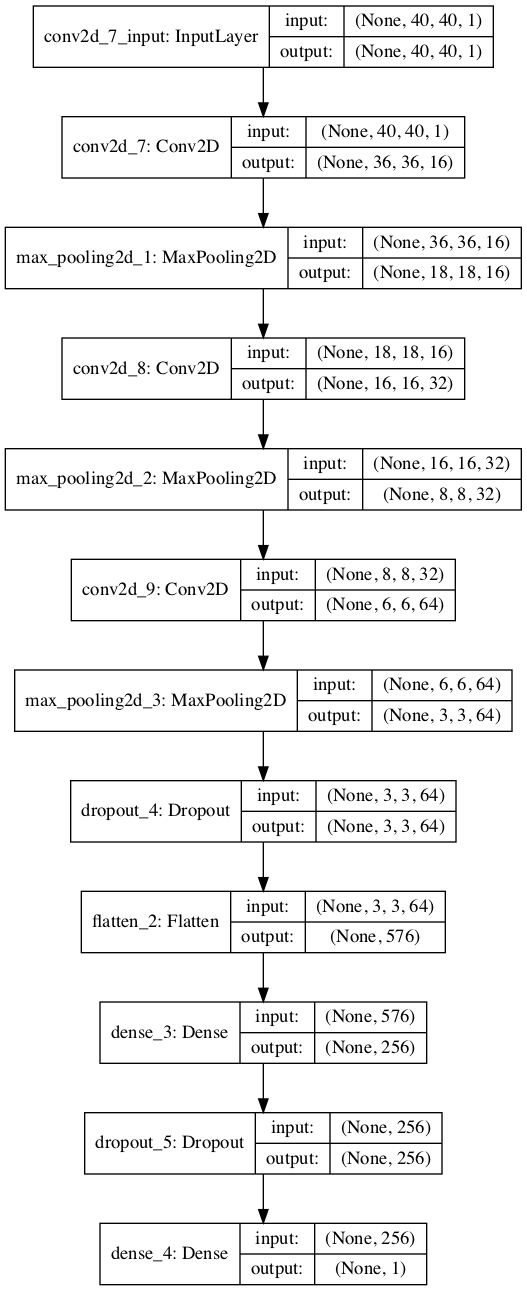
\includegraphics[width=\columnwidth]{../Figures/CNN_model_self} 
 \caption{CNN made from scratch}
 \label{fig:ScratchCNN}
 \end{subfigure}
 \begin{subfigure}{0.8\columnwidth}
 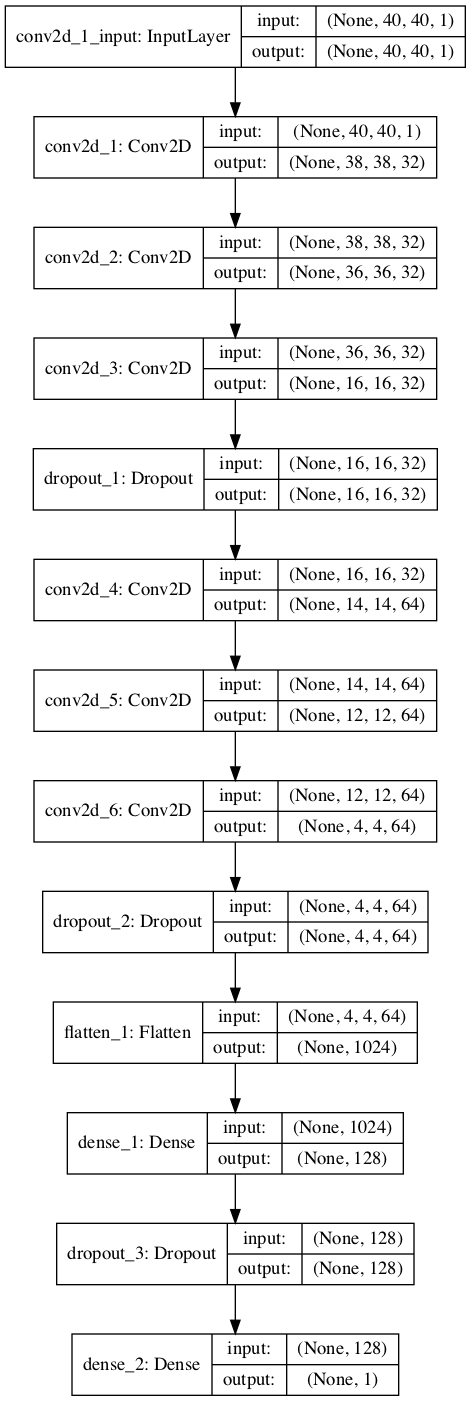
\includegraphics[width=\columnwidth]{../Figures/CNN_model}
 \caption{CNN referencing the MNIST Kaggle CNN}
 \label{fig:MNISTCNN}
 \end{subfigure}

\caption{These are the CNN architectures used within the project. Fig.~\ref{fig:ScratchCNN} represents the architecture made from scratch. Note the use of pooling layers in between convolutional layers. These pooling layers are used to reduce the dimensionality of the data, thereby reducing the computation time. Fig.~\ref{fig:MNISTCNN} represents the architecture used in the MNIST Kaggle CNN. Note the absence of pooling layers. It can be said that the pooling layers in this case are replaced with more convolutional layers. At certain layers, namely \texttt{conv2d\_3} and \texttt{conv2d\_6}, the output dimensions drop by approximately half compared to the input dimensions. This looks similar to the pooling layers in Fig.~\ref{fig:ScratchCNN} but are in fact convolutional layers with a stride length of 2. This means that the convolutional filter skips over every other pixel in the process of convolution, thereby forming a convolutional image on the order of half the input image. This also has the effect of a layer which reduces the dimensionality, but also allows the layer's connections to be trained. This means that the number of trainable parameters are increased in this model but also calls for longer computational time. \label{fig:CNNArchitecture}}
 
 \end{figure*}

\subsubsection{Optimisers}
There are a variety of optimisers available for selection within the neural network package used. Because most modern implementations of neural neural networks use some kind of adaptive gradient, initially AdaDelta was chosen as the optimiser. However, the accuracy reached using AdaDelta was not as good expected, therefore the Adam optimiser was used instead. This yielded good results, but also would occasionally return meaningless results of 50\% accuracy---50\% accuracy means a classifier which does no better than random chance. The reason for this is probably due to the momentum aspect of Adam---i.e. it accumulates too much momentum and doesn't manage to stop in the minimum. However, the solution to this, as described in the above section \ref{section:modern optimizers}, a solution which was a modification to the Adam algorithm---AMSgrad was released in 2018. This modification is also implemented in the neural network packaged used hence it was directly used. The result is that the neural networks using Adam and AMSgrad all converge, and contrary to some preliminary findings, there was no appreciable decrease in performance (convergence time). 

The neural networks were trained for 1024 epochs, with a batch size of 32. This means that each batch includes 32 randomly selected images that have not been previously selected in the batch and the whole dataset was 'run through' 1024 times for the duration of the training. 

\subsection{Data Augmentation}
One key areas that is discovered in the generation of cutout images is that vastly more stars than galaxy are present in the dataset. So far, because equal number of each class must be preserved, a majority of stars are discarded and not used for training. This seems unsatisfactory and wasteful, therefore data augmentation was performed on the images. Data augmentation is the process of artificially increasing the amount of data available to train with. The data augmentation performed on the galaxy images. Because galaxies on the sky can appear in any orientation, the galaxy images were rotated by 90,180,270 degrees to form 3 additional images, and each of these, including the original one was reflected along one axis to form a total of 8 times more galaxy images. Given that there are now 8 times as many galaxy images as before, 8 times as many stellar images may be used. This gives a total of 49968 images in total and therefore 39974 images to train with. Because there is a wealth of stellar images, the increased images may be taken directly, and hence are unique images. The results of training using data acquired from this process are detailed below. 
\section{Results}
\subsection{Quantifying Results}
In discussing the results, there are a few ways to quantify the quality of the classifier. The quantified performance of the classifier should also be balanced against the time it takes to train. To determine the goodness of the classifier, one should use metrics to determine how well the classifier classifies. Here, since this is a binary classifier, there are a  number of well established metrics which can be used. 

A confusion matrix is a matrix which groups the results of the classification into whether they are classified correctly or not. In a binary classifier, the confusion matrix has the form $CM=\begin{bmatrix}
           TP & FP \\
           FN & TN \\
         \end{bmatrix}$ , where TP stands for 'True Positive', which is the number of correctly classified 'positive' datapoints---in this project, since the purpose is to find galaxies, galaxies will be assigned as 'positive' results, the opposite assignation can be done with no loss in validity and will result in a transposed version of the same matrix. TN stands for 'True Negative', which is the number of correctly classified 'negative' datapoints---here stars. FP are 'negative' datapoints which the classifiers misclassify as positive---a star which the classifier classifies as galaxies, and finally FN is the opposite---an image of a galaxy which is misclassified as a star. In general, a good classifier should have a high $\frac{tr(CM)}{\sum{CM}-tr(CM)}$, where $tr(CM)$ is the trace of the confusion matrix, and $\sum{CM}$ is the sum of all elements in the confusion matrix. In essence, this quantity is the ratio of correctly classified datapoints to incorrectly classified datapoints. From this, more metrics could be defined to better quantify the performance of the classifier. 
         
 One of the most common metrics used is accuracy. It is defined as 
 \begin{equation}
 	ACC=\frac{TP+TN}{P+N}
 \end{equation}
  where P is the total number of Positive datapoints in total, and N is the total number of Negative datapoints in total. This is very intuitive as this is simply the percentage of the total amount of correct classifications. NB: A corresponding metric called the error rate is simply 1-Accuracy. Accuracy as a metric is generally good enough for most general classification purposes. However, there are cases, such as unbalanced datasets or when the purity of the prediction is important, where other metrics are important. 
  
  Sensitivity (or recall or true positive rate) is defined as follows
  \begin{equation}
  SN=\frac{TP}{P}	
  \end{equation}
This metric shows the fraction of correctly classified positive datapoints in all positive datapoints. This metric is important when the positive dataset is very small, such as when looking at a rare signal in a large amount of noise. 

  Precision (or positive predictive value) is defined as follows
  \begin{equation}
  PREC=\frac{TP}{TP+FP}	
  \end{equation}
This metric shows the fraction of correctly classified positive datapoints in all datapoints predicted as positive. This metric is important when the purity of the positive classified dataset is important.

From these 3 metrics and the confusion matrix itself, a further refinement/development of classification metrics can be developed. Matthews Correlation Coefficient is a metric which takes into account both the positive and negative classification. \cite{MCC} It is defined thus
\begin{equation}
MCC = \frac{TP\times TN - FP\times FN}{\sqrt{(TP+FP)(TP+FN)(TP+FP)(TN+FN)}}	
\end{equation}
The Matthews Correlation Coefficient ranges from -1 to 1, where a coefficient of 1 represents a perfect classifier while a coefficient of -1 represents a classifier which assigns positive classification to all negative values and vice versa. A coefficient of 0 represents a random classifier. This coefficient has its roots in statistical theory and is related to the phi coefficient which is in turn related to the chi-squared statistic. When the confusion matrix is seen as a 2x2 contingency table, the relation is as follows
\begin{equation}
|MCC| = \phi = \frac{\chi^2}{n}
\end{equation}
where n is the total number of items in the contingency table. 

The F-score is a score which only takes into consideration the positive classification. There are many F-scores, all of which are harmonic means of precision and sensitivity. \citep{F1} It is defined as follows
\begin{equation}
F_\beta = \frac{(1+\beta^2)(PREC\cdot SN)}{\beta^2 \cdot PREC + SN}
\end{equation}
The most used F-score is the $F_1$ score. 
\begin{equation}
F_1 = \frac{2(PREC\cdot SN)}{PREC + SN}
\end{equation}
$F_1$ ranges from 0 to 1, where a score of 1 represents a classifier which classifies all positive datapoints as positive but no others. A score of 0 represents the classifier did not classify any positive datapoints as positive. As one can see, this metric only accounts for the positive classifications and neglect the negative classifications entirely. 

Therefore the $F_1$ score is more appropriate when only the positive class is important---in this project, if one were only to be interested in extracting only galaxies in the image, for example. The Matthews Correlation Coefficient is important when one requires correct classifications for both classes---in this project, if one is performing a statistical study of all the stars and galaxies in the field, for example. 

Below, the accuracy, $F_1$ score and the Matthew Correlation Coefficient will be tabulated below for the FNN model, the CNN model built from scratch, the CNN model from studying the MNIST model, the CNN model built from scratch with data augmented, and the CNN model from studying the MNIST model with data augmented. See Table \ref{table:results}.


\begin{table*}
 \begin{tabular}{||c|c c c |c||} 
 \hline
  & Accuracy & $F_1$ Score & Matthews Correlation Coefficient & \makecell{Median Time to \\Complete 1 Epoch (s)}\\ [0.5ex] 
 \hline\hline
 FNN model & 85.760\% & 85.668\% & 71.521\%  & 0.068\\ 
 \hline
 CNN model built from scratch & 91.760\% & 91.633\% & 83.519\%  & 1.065\\
 \hline
 CNN model from studying the MNIST model & 92.880\% & 92.477\% & 85.940\% & 1.173 \\
 \hline
  CNN model built from scratch with data augmented & 93.116\% & 93.043\% & 86.254\% & 4.095\\
 \hline
 CNN model from studying the MNIST model with data augmented & 93.926\% & 93.798\% & 87.935\% & 7.176\\
 \hline
\end{tabular}
\caption{Table of results gained from the 5 different configurations of models used. Accuracy, $F_	1$ score, Matthews Correlation Coefficient and median time to train 1 epoch given. Note that $F_1$ Score and Matthews Correlation Coefficient are not usually given in \%, but usually in decimal---i.e. 0.9 rather than 90\% because they are not fractions of a whole. But to unify the representation, they have been converted to \%. The underlying meaning should be clear. Matthews Correlation Coefficient and $F_1$ Score should not be directly compared because, first, the range of the Matthews Correlation Coefficient is twice that of $F_1$ score, and second, the two metrics are measuring different things which are not directly related. The accuracy is the most often cited metric to compare, but it is more fruitful to compare either the Matthews Correlation Coefficient or the $F_1$ Score depending on the purpose of the classifier. The results indicate that augmented data is better than non-augmented data, and that CNNs are more fit for purpose than FNNs. The median time to complete 1 epoch of training also relates to the model as expected---the more complex the model the longer it takes to train and the larger the dataset, the longer it takes to train. However, the ratio is not as expected, with 8 times the amount of data, the difference in training time is only by a factor of 4-6. This is probably due to the overhead which is fixed for every epoch. \label{table:results}}
\end{table*}
However, the time it takes to train the model should not be neglected. There is a very real tradeoff between specific performance and the time it takes to train the model. Because each of the models are trained for the same 1024 epochs, the time to train is based on completing these 1024 epochs rather than the somewhat more useful metric of time taken to reach a certain accuracy. However, this metric has its value in determining the computational complexity of training each one of those models. 
\subsection{Discussion}
These results indicate that the CNN models are clearly superior to the FNN models at classifying images, which is expected. The sole advantage the FNN model has over the CNN models is the training time, which is over a magnitude faster. However, given that an accuracy of 85.7\% is not sufficient to have any practical use whatsoever, it can be conclusively determined that CNNs are the way forward in terms of astronomical morphological classification. 

Models trained on augmented data seem to perform slightly better across the board in comparison to models not. The models trained on augmented data seem to outperform the models trained on non-augmented data by about 1\%. This minor increase in performance is probably due to the fact that augmenting data does not actually increase the variance (amount of information in the images) in the galaxy images. However, this difference is not conclusively separated from statistical variance as there is some inherent randomness between models-runs because the initial random seed is different. However, using augmented data means increasing the amount of data trained by 8 times, which correspondingly increases training time significantly. Therefore, augmenting one class of data to train with is generally inadvisable. A better approach would be to assign different weighting to training each class which would enable the use of unbalanced datasets. This would entail using most of the data even though stars vastly outnumber galaxies. In this case, misclassifying a galaxy would carry a much higher loss than misclassifying a star, because galaxies much rarer in the dataset. This would, however, increase the complexity of the code significantly. 

Another thing of note here is that the $F_1$ score and Matthews Correlation Coefficient seems to vary together in each dataset and model---the MNIST CNN with augmented data has the highest metric in each category (along with taking the longest to train), while the CNN from scratch without data augmentation has the lowest metric (FNN notwithstanding). This indicates that no one model is especially suited to extracting galaxies which is a speculative use for a model like this, and that the MNIST CNN with augmented data is generally the best model.

The threshold for this model is set at 0.5. On deeper inspection, it is found that the model tends to yield very extreme results. See Fig.~\ref{fig:probability} This means that moving the threshold would not be very useful in increasing the precision in detecting galaxies. This means that to improve this model, it is not as simple as moving the threshold. 

\begin{figure}
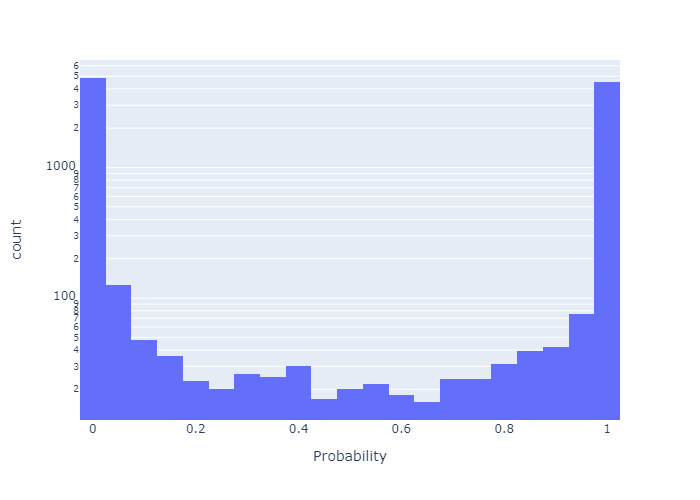
\includegraphics[width=\columnwidth]{../Figures/probability}
\caption{The resulting probabilities are very extreme. The vast majority of the probabilities are very close to 0---prediction of a star, or close to 1---prediction of a galaxy. NB: The scale is a logarithmic scale which shows how pronounced the peaks are. This makes it difficult to make any kind of progress by simply moving the threshold. Therefore, the threshold is set at 0.5, but it would not make a large difference whether it is any number from 0.2 to 0.8. \label{fig:probability}}
\end{figure}


Ultimately, in the best case result, the model yields a classification accuracy of 94\% and a Matthews Correlation Coefficient in the region of 88\%. This is not good enough for doing catalogue classification as there are a sizeable portion of impurities in both classifications. However, this shows that neural networks currently are good to use as tool for performing a 'first-pass' approach towards new datasets because this weeds out a great majority of incorrect datapoints. If a purer sample is required, one simply has to select from the classes given by the classifier because the datasets after classification is much denser in the desired class. A practical example is that if one were to want to study galaxies, after classification by this neural network, one only has to select galaxies from the galaxy class in this neural network. This is much easier than selecting from the overall dataset because the dataset is much small here and also much closer to a pure sample so one has to examine a much smaller number of images to reach the desired number of samples. 

It is a well established problem in astronomical machine learning that the final 5\% accuracy (increasing accuracy above 95\%) is hardest to achieve. This is due to the fact that objects in the sky are naturally ambiguous, such as those seen in Fig.~\ref{fig:Examples}. If even a human has trouble distinguishing between those objects, then it is reasonable to expect a machine to do much better. This problem is also related to the fact that wide field telescopes do not represent a high resolution image often needed to conclusively distinguish between a star and a galaxy. Studies done using higher resolution images have better results, such as \citet{Khalifa2017} who achieved over 97\% accuracy in the harder problem of distinguishing between galaxy types because they used multi-channel imagery as well as higher quality imagery. 

A study done on data of similar quality to this project by \citet{Aniyan2017} yielded a much more modest $F_1$ Score of 0.91 for classifying galaxies. Note that the $F_1$ Score calculation is mine, they provided the precision and recall which is sufficient to calculate the $F_1$ Score. 

A direct comparison can be made with \citet{Kim2016} as that was a study done on star-galaxy classification using CNNs. They achieved a maximum $F_1$ Score of 0.9603 ($F_1$ calculation here mine). This is significantly better than the $F_1$ Score achieved in this project which indicates that there should be significant optimizations available to made in the future.

\section{Future Improvements}
A key source of possible improvement is adding more data to train the model. At the moment, there is no lack of data, since data the data required to train the model is simply images which is captured by GOTO, but also in the SDSS catalogues. The overlap of these datasets are quite large and so there is no lack of data here. 

A concern at large datasets, however, is a memory problem. Since computers have finite RAM, at large datasets, the size of the dataset would frequently exceed the RAM of a regular computer. The train-test split approach relies on loading the entire dataset into RAM before performing operations on it. This would not work if the dataset exceeds RAM size. In research applications, the hardware is usually either processing speed bound (CPU and GPU are limitation, while RAM is effectively unlimited), or memory bound (RAM is limited, while processing power is very high, usually by way of CPUs with very high core counts). In processor-bound applications, the train-test split is appropriate because RAM is faster than loading from disk and has the benefit of knowing what the entire dataset looks like beforehand and therefore allows for some preprocessing. In memory-bound applications however, the train-test split does not work and instead an alternative method must be sought. A popular method for image recognition is the dataloader approach. \citep{Dataloader} This approach only retrieves images which are needed for the specific training batch and therefore the memory requirements are much smaller, but has a trade off of requiring much more processing power as well as needing a fast storage medium (SSD, or even RAM based storage like Intel Optane is ideal). 

With respect to the network architecture, the exact architecture that is best for the dataset varies per dataset. It is highly unlikely that any of the architectures used in this project is the optimal one. To determine the best network architecture, either a manual approach is needed to tune the hyperparameters (numbers of layers, numbers of nodes in each layer, activation algorithms, dropout ratios, etc.) of the network. This frequently entails using a validation set data. Since, the MNIST model was used directly, this process was omitted but probably have yielded some improvement in performance. This process is highly time consuming as the model needs to be retrained over each iteration of the network architecture. Some very new packages such as Google's AutoML \citep{AutoML}, and the open source AutoKeras \citep{AutoKeras} have this training functionality inbuilt. But due to package incompatibility issues which are unresolvable until a new patch is released, this path could not be explored, but in the future this may well be the way forward. 

In the field of survey astronomy, there is some interest in using unsupervised algorithms---i.e., algorithms which do not require labeled data to classify objects. These has the obvious benefit of not requiring labeled data which, in some cases may be hard to come by. A second benefit of working with unsupervised algorithms is that they allow for the discovery of classes of objects which previously astronomers thought were parts of other classes or that previous divisions in classes are not supported by the data. This gives an objective method of creating classes of objects for which there may or may not be a physical basis to exist. A very good example of this would be \citet{Hocking2018}.

\section{Conclusion}
This project proves the viability of using a neural network classify to assist in the work of survey astronomy. An example of how this neural network could be implemented is provided. In the future, it may be possible to completely automate the classification process in catalogues, but this is not possible at the current stage. This project also illustrates the challenges in this area frequently lie in issues yielding labeled data instead of the actual usage of that data. Once labeled data is created, extant computer science techniques are readily available to be applied to this data to create a classifier. Machine classifications of survey astronomy images is an eminently feasible endeavour, with machine classifications of catalogue objects not too far in the future. This has the possibility of drastically increasing the possible size of catalogues because one of the most time consuming steps has been automated.

Over the course of conducting this project, a number of pitfalls which have been found are that software compatibility is a vital aspect of any coding task. Most of the time spent on working on high level code (such as what Keras provides), is whether the package works in your existing environment and what methods can be used to harmonise them. Another aspect of working with high level code is that often, if something fails to work as one intends, there is no easy fix because the root cause is buried within the lower level implementation which working with the higher level code seeks to avoid. A prime example of this would be the GPU implementation of Keras---since Keras relies on Tensorflow (in this project) as its backend, the Keras GPU implementation is actually the Tensorflow implementation. If that fails to work, then the code which is possibly faulty lies in the Tensorflow source code, which is written in very complex C++. However, overall, working with high level code is an easily accessible way for non-computer scientists to access the tools of machine learning, hence, the prospects of machine learning in astronomy should only grow over time. 

\section*{Acknowledgements}
Thanks to Dr James Mullaney for his thoughtful criticism, comments and guidance throughout the course of the project. This project would not have been successful if not for his often timely interventions to prevent time being wasted on a dead end. Thanks also to Lydia Makrygianni who found and uploaded GOTO images which was also covered by SDSS. The images formed the basis of this entire project and without them the project wouldn't have even gotten off the ground.

% References
%
% The best way to enter references is to use BibTeX:

\bibliographystyle{mnras}
\bibliography{Sem2}


% Alternatively you could enter them by hand, like this:
% This method is tedious and prone to error if you have lots of references

%\begin{thebibliography}{99}
% The 99 argument allows you to have up to 99 references. If you have more than 99 (not recommended!), you will need to change it to 999.




%\end{thebibliography}


\appendix

\section{Semester One Project Plan}
\label{App:project plan}
\subsubsection{Postage Stamp Cutout}
Small 'postage stamp' cutouts from the large image are required to train SVMs. This requires that the previous source detection algorithm is functional. I believe this will take up to 10 hours. 
\subsubsection{Cross-Referencing Data}
After a satisfactory set of postage stamps is acquired, the cutouts need to be cross referenced with existing sky surveys to identify known objects to use as a training set. For now, the plan is to use SDSS to be the primary catalogue of reference. This should take up to 10 hours.
\subsubsection{PCA}
Performing a PCA on the data should be straightforwardly applying the algorithm. The issue is computing time, but I don't foresee this taking a vast amount of that either. I will allocate 5 hours to this for the time being.
\subsubsection{SVM and Kernal SVM}
Once the PCA is complete, a simple SVM can be performed, either using packaged algorithms or self-written ones. The limiting factor here is also computing time since an SVM algorithm is quite straight-forward to write.
Once that is complete, a kernal-SVM algorithm will be attempted. However since this is quite complex, a packaged solution will probably be used. I foresee many potential issues with trying this so I would allocate a total of 25 hours for this section.
\subsubsection{CNN}
After the SVM/PCA method is completed, a CNN will be attempted. Since the allure of a CNN is that it does not require the cutting out of postage stamps, that will be the first choice. However, it is still difficult to see how to properly make a training set for CNN this way. Further, many refinements would be necessary for a CNN, and training each iteration will be very time intensive. Therefore, I will conservatively estimate that 60 hours will be needed.
\subsubsection{Report}
After the project proper is finished, the report will be written. I expect some 10-20 hours will be spent on report writing.
\subsubsection{Other areas}
If there is any time to spare, other possible areas of work would be to make a Feedforward Neural Network and compare the results to kSVM. Otherwise, if the project proceeds vastly better than expected, an attempt to classify galaxies can be done.

\subsection{Review on Project Plan}
Overall, the project achieved what it set out to achieve---make a classifier to distinguish stars and galaxies. The amount of time spent on each section changed greatly compared to the project plan. The postage stamp and cross referencing data section of the plan took up to 60 hours of work to complete. This was a vast underestimation of the time it takes to complete this. At the same time, however, it was a trivial task to do once the method to do so was established. The extra time spent meant that the PCA and SVM plans had to be removed completely and work began on an FNN. 

The FNN took over 10 hours to complete and didn't have the desired effect, therefore the focus changed to CNNs which was part of the initial plan. The CNN took a long time, mostly due to the long training times of the CNN as well as software bugs and glitches. The CNN section of the project took up to 100 hours of my time.

In terms of software issues, I ran into multiple instances where my GPU would not be detected and there's nothing I could do except uninstall and reinstall my entire Anaconda python which was both laborious and time consuming (somewhat due to slow internet). I also ran into multiple instances where a certain package would not work on windows and therefore I had to create some of my graphics on another machine which was another timesink. Finally, a software update in the middle of the project rendered some of the vital packages unusable. This, in particular, was only solved by uninstalling and reinstalling an old version of Anaconda from scratch. Overall, the most unexpected time loss went to these software issues. I believe most of them could be mitigated with working in a virtual environment, but at the time it seemed more trouble than it was worth. 

Finally, the report took substantially longer than 10-20 hours, in fact, report writing took, on the order of 45-50 hours. This meant that there was no time to explore making a CNN which distinguished between spiral and elliptical galaxies as was a stretch goal in the plan.
\section{Effect of industrial action and coronavirus}
\label{2020 special}
The coronavirus epidemic meant that I traveled back to my home country of Hong Kong in late March. When I arrived, I was subject to 14 days of home quarantine with no broadband internet. However, this was mitigated somewhat by using mobile data, but was not ideal. This also meant that project meetings needed to be scheduled at night time here, but this was by no means insurmountable. The coronavirus which also meant that the PhD student (Lydia) had provided the GOTO data and placed it online was subsequently unavailable, hence only 32 GOTO images was used to train the data and exploring increasing the dataset was impossible. 


\section{Source Code}
\label{Code}
The code used in this project can be found at the GitHub repository: \url{https://github.com/kpklo1/Machine-Learning-and-Galaxies}

\section{Hardware and Software Packages Used}
\label{HSWare}
\subsection{Hardware}
This was the specifications of the hardware used:

Laptop 1
\begin{itemize}
\item OS: Windows 10 Professional
\item CPU: Intel Core-i9 9900HK running at 3.6GHz (8-core)
\item GPU: GTX 2080 at base clock
\item RAM: 32GB DDR4
\end{itemize}

Laptop 2
\begin{itemize}
\item OS: MacOS Catalina 10.15.1
\item CPU: Intel Core-i7 6920HQ running at 2.9GHz (Quad-core)
\item GPU: Irrelevant because software does not support non-CUDA cards
\item RAM: 16GB LPDDR3
\end{itemize}

\subsection{Software}
\begin{itemize}
\item Anaconda 2019.10
\item Python 3.7.6
\item Numpy 1.18.1
\item Astropy 4.0
\item Tensorflow 2.1.0
\item Pandas 1.0.1
\item sklearn 0.22.1
\item photutils 0.7.2
\item Keras 2.3.1 (Using Tensorflow backend)	
\end{itemize}

\section{Miscellaneous Figures}
\label{ExtraFigs}
Some figures were produced during the course of making the report but were not used in the body of the text. However, I feel it may be useful to include them nonetheless as they may shed light on some aspects of the project which remains unclear in the body. 

\begin{figure*}

 \begin{subfigure}{\columnwidth}
 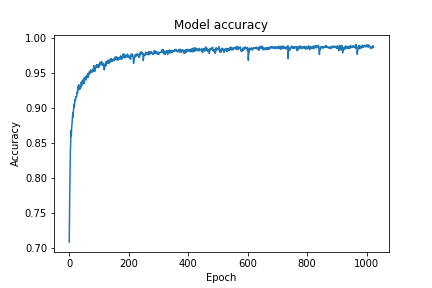
\includegraphics[width=\columnwidth]{../Figures/CNN_self} 
 \caption{CNN from Scratch}
 \label{fig:CNN_self}
 \end{subfigure}
 \begin{subfigure}{\columnwidth}
 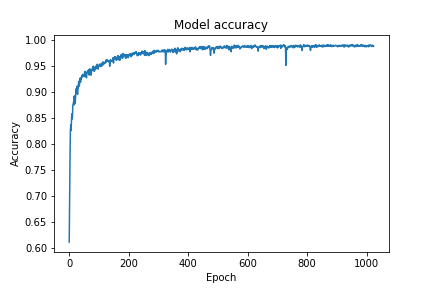
\includegraphics[width=\columnwidth]{../Figures/CNN_MNIST}
 \caption{MNIST CNN}
 \label{fig:CNN_MNIST}
 \end{subfigure}
 \begin{subfigure}{\columnwidth}
 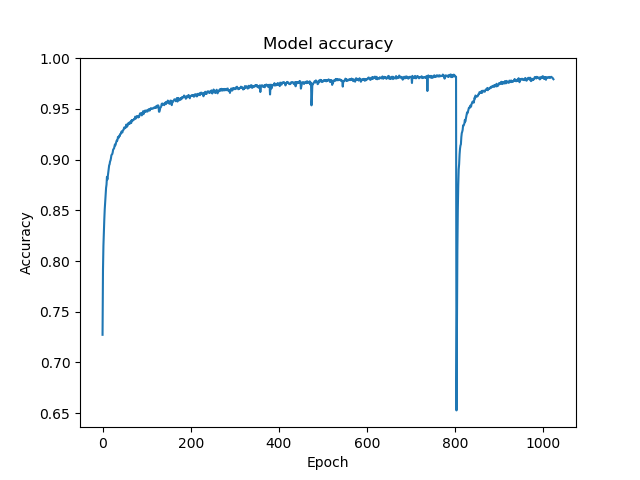
\includegraphics[width=\columnwidth]{../Figures/CNN_Augment_Self}
 \caption{Data Augmented CNN from Scratch}
 \label{fig:CNN_Augment_Self}
 \end{subfigure}
  \begin{subfigure}{\columnwidth}
 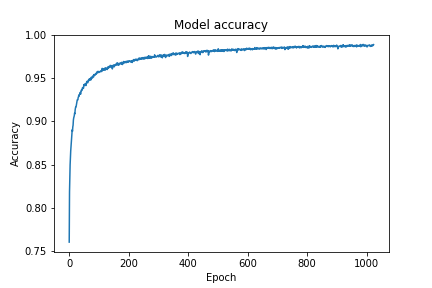
\includegraphics[width=\columnwidth]{../Figures/CNN_Augment_MNIST}
 \caption{Data Augmented MNIST CNN}
 \label{fig:CNN_Augment_MNIST}
 \end{subfigure}

 \caption{These are a series of graphs showing the convergence of the CNN models over epoch. Of note is Fig.~\ref{fig:CNN_Augment_Self}, where the accuracy dropped to 0.65 but returned to convergence. I do not have an explanation for this. It may be a statistical fluke, or a bug in the program.}
 \label{fig:Examples}
 \end{figure*}


\section{Miscellaneous Items}
\label{Misc}
Due to the fine nature of the images in this report, the report is best viewed digitally instead of on print. 

% Don't change these lines
\bsp	% typesetting comment
\label{lastpage}
\end{document}

% End of mnras_template.tex













